\documentclass[NET,english,beameralt]{tumbeamer}

% If you load additional packages, do so in packages.sty as figures are build
% as standalone documents and you may want to have effect on them, too.

% Folder structure:
% .
% ├── beamermods.sty                  % depricated an will be removed soon
% ├── compile                         % remotely compile slides
% ├── figures                         % all figures go here
% │� �  └── schichtenmodelle_osi.tikz   % each .tikz or .tex is a target
% ├── include                         % create your document here
% │� �  ├── example.tex                 % example document
% │� �  └── slides.tex                  % make document wide changes here
% ├── lit.bib                         % literature
% ├── Makefile
% ├── moeptikz.sty                    % fancy networking symbols
% ├── packages.sty                    % load additional packages there
% ├── pics                            % binary pcitures go here
% ├── slides.tex                      % main document (may be more than one)
% ├── tumbeamer.cls
% ├── tumcolor.sty                    % TUM color definitions
% ├── tumcontact.sty                  % TUM headers and footers
% ├── tumlang.sty                     % TUM names and language settings
% └── tumlogo.sty                     % TUM logos

% Configure author, title, etc. here:
\documentclass[NET,english,beameralt]{tumbeamer}

% If you load additional packages, do so in packages.sty as figures are build
% as standalone documents and you may want to have effect on them, too.

% Folder structure:
% .
% ├── beamermods.sty                  % depricated an will be removed soon
% ├── compile                         % remotely compile slides
% ├── figures                         % all figures go here
% │� �  └── schichtenmodelle_osi.tikz   % each .tikz or .tex is a target
% ├── include                         % create your document here
% │� �  ├── example.tex                 % example document
% │� �  └── slides.tex                  % make document wide changes here
% ├── lit.bib                         % literature
% ├── Makefile
% ├── moeptikz.sty                    % fancy networking symbols
% ├── packages.sty                    % load additional packages there
% ├── pics                            % binary pcitures go here
% ├── slides.tex                      % main document (may be more than one)
% ├── tumbeamer.cls
% ├── tumcolor.sty                    % TUM color definitions
% ├── tumcontact.sty                  % TUM headers and footers
% ├── tumlang.sty                     % TUM names and language settings
% └── tumlogo.sty                     % TUM logos

% Configure author, title, etc. here:
\documentclass[NET,english,beameralt]{tumbeamer}

% If you load additional packages, do so in packages.sty as figures are build
% as standalone documents and you may want to have effect on them, too.

% Folder structure:
% .
% ├── beamermods.sty                  % depricated an will be removed soon
% ├── compile                         % remotely compile slides
% ├── figures                         % all figures go here
% │� �  └── schichtenmodelle_osi.tikz   % each .tikz or .tex is a target
% ├── include                         % create your document here
% │� �  ├── example.tex                 % example document
% │� �  └── slides.tex                  % make document wide changes here
% ├── lit.bib                         % literature
% ├── Makefile
% ├── moeptikz.sty                    % fancy networking symbols
% ├── packages.sty                    % load additional packages there
% ├── pics                            % binary pcitures go here
% ├── slides.tex                      % main document (may be more than one)
% ├── tumbeamer.cls
% ├── tumcolor.sty                    % TUM color definitions
% ├── tumcontact.sty                  % TUM headers and footers
% ├── tumlang.sty                     % TUM names and language settings
% └── tumlogo.sty                     % TUM logos

% Configure author, title, etc. here:
\documentclass[NET,english,beameralt]{tumbeamer}

% If you load additional packages, do so in packages.sty as figures are build
% as standalone documents and you may want to have effect on them, too.

% Folder structure:
% .
% ├── beamermods.sty                  % depricated an will be removed soon
% ├── compile                         % remotely compile slides
% ├── figures                         % all figures go here
% │� �  └── schichtenmodelle_osi.tikz   % each .tikz or .tex is a target
% ├── include                         % create your document here
% │� �  ├── example.tex                 % example document
% │� �  └── slides.tex                  % make document wide changes here
% ├── lit.bib                         % literature
% ├── Makefile
% ├── moeptikz.sty                    % fancy networking symbols
% ├── packages.sty                    % load additional packages there
% ├── pics                            % binary pcitures go here
% ├── slides.tex                      % main document (may be more than one)
% ├── tumbeamer.cls
% ├── tumcolor.sty                    % TUM color definitions
% ├── tumcontact.sty                  % TUM headers and footers
% ├── tumlang.sty                     % TUM names and language settings
% └── tumlogo.sty                     % TUM logos

% Configure author, title, etc. here:
\input{include/slides}

\renewcommand{\chairname}{Chair of Connected Mobility}

\begin{document}

% If you are preparing a talk but do not like the default font sizes, you may
% want to try the class option 'beameralt', which uses smaller default font
% sizes and integrates subsection/subsubsection names into the headline.

% For lecture mode, you may want to build one set of slides per chapter but
% with common page numbering. If so,
% 1) create a new .tex file for each chapter, e.g. slides_chapN.tex,
% 2) set the part counter to N-1 (assuming chapters start at 0), and
% 3) and name your chapter by using the \part{} command.
%\setcounter{part}{-1}
%\part{Organisatorisches und Einleitung}

% For 16:9 slides, use the class option 'aspectratio=169'.

% If class option 'noframenumbers' is given, frame numbers are not printed.

% If class option 'notitleframe' is given, the title frame is not autmatically
% generated.

% Class option 'nocontentframes' suppresses automatic generation of content
% frames when new parts/sections are started.

% Include source files from ./include (or ./include/chapN).
\input{include/agenda}
\input{include/introduction}
\input{include/background}
\input{include/results}
\input{include/conclusion}

% Include markdown source from ./pandoc
%\input{pandoc/example}

% Comment out if you do not want a bibliography
\section{Bibliography}
\begin{frame}[allowframebreaks]
    \bibliographystyle{abbrv}
    \setbeamertemplate{bibliography item}[text]
    \footnotesize
    \bibliography{lit}
\end{frame}

\end{document}



\renewcommand{\chairname}{Chair of Connected Mobility}

\begin{document}

% If you are preparing a talk but do not like the default font sizes, you may
% want to try the class option 'beameralt', which uses smaller default font
% sizes and integrates subsection/subsubsection names into the headline.

% For lecture mode, you may want to build one set of slides per chapter but
% with common page numbering. If so,
% 1) create a new .tex file for each chapter, e.g. slides_chapN.tex,
% 2) set the part counter to N-1 (assuming chapters start at 0), and
% 3) and name your chapter by using the \part{} command.
%\setcounter{part}{-1}
%\part{Organisatorisches und Einleitung}

% For 16:9 slides, use the class option 'aspectratio=169'.

% If class option 'noframenumbers' is given, frame numbers are not printed.

% If class option 'notitleframe' is given, the title frame is not autmatically
% generated.

% Class option 'nocontentframes' suppresses automatic generation of content
% frames when new parts/sections are started.

% Include source files from ./include (or ./include/chapN).
\section{Agenda}

\begin{frame}
    \begin{itemize}
        \item Motivation \& Summary of Original Paper
        \item Background: Web Performance Metrics \& Tools
        \item Re-Implementation \& Results
        \item Conclusion
    \end{itemize}
\end{frame}

\section{Motivation \& Summary of Original Paper}

\begin{frame}
    \frametitle{Motivation}
    Web browsing is one of the most widely-used applications used in today's Internet ecosystem. A number of metrics have been developed and used as benchmarks to accurately reflect the performance of web applications for users. \textbf{Measurements can differ greatly depending on a number of factors:}
    \begin{itemize}
        \item Surveyed Web Pages
        \item User Devices
        \item Browsers
        \item Tools (e.g. Selenium)
        \item Metrics
    \end{itemize}
    $\boldsymbol{\rightarrow}$ This diversity as well as the lack of clearly established standards lead to difficulties when quantifying performance. The original paper \cite{10.1007/978-3-030-15986-3_19} examined the effects of these ambiguities with regards to browsers, tools, and metrics and provided guidelines for future papers.
\end{frame}

\begin{frame}
    \frametitle{Summary of Original Paper}
	The original paper \cite{10.1007/978-3-030-15986-3_19} was structured as follows:
    \begin{enumerate}
        \item Introduction
        \item Metric Definitions \& Tools
        \item Survey of 15 Web Studies
        \item Methodology
        \item Identification of Pitfalls \& Guidelines for Future Papers
    \end{enumerate}
\end{frame}
\section{Background}
\label{sec:background}
Among the most important web metrics are load times, number \& size of objects, and page size. Each of the aforementioned metrics can be measured according to numerous definitions and using data from diverse data sources. The following section provides an overview of these definitions and the data sources used in this paper.

\subsection{Load Times}
The time required for loading a web page correlates strongly with user experience \cite{6263888}. A browser normally loads a web page in multiple steps: load and parse the base document, construct a Document Object Model (DOM), load and process referenced objects, render / display the results. Although Page Load Time (PLT), defined as the time until the onLoad event, is most often used to measure page load times, there are a number of other metrics. For example, Time To First Paint (TTFP) and Above The Fold Time (AFT) are triggered before PLT when the content is first displayed and available to the user. The start times used for calculating load times can always differ (e.g. navigationStart, fetchStart). One of the main takeaways from \cite{10.1007/978-3-030-15986-3_19} is that redirects can strongly affect these measurements and should be accounted for; Figure \ref{fig:plot_redirects} shows the impact redirects can have on PLT and Figure \ref{fig:bar_redirects} the prevalence of such redirects. 

There is also a plurality of data sources for calculating load times. The standardized API for navigation timings \cite{timing_2012} is used to fetch load times based on browser events. It is important to note that events / metrics provided by the Navigation Timings API are not necessarily defined in the same way for all browsers. HTTP Archive files \cite{har_format_2012} and the Resource Timings API \cite{w3c_2020} also provide load time data. The majority of modern browsers (e.g. Chrome, Firefox) implement the Navigation Timings and Resource Timings APIs; HAR files can be exported using developer tools. Both Chrome and Firefox provide remote debugging and page load automation interfaces (i.e. Chrome DevTools \& Firefox Marionette). There are also third-party automation frameworks that allow for the same basic functionality as well as extended functions (e.g. keyboard input); Selenium, one of the most popular such tools, is used in the original paper.

 \begin{figure}
 \centering
 \begin{subfigure}{\linewidth}
		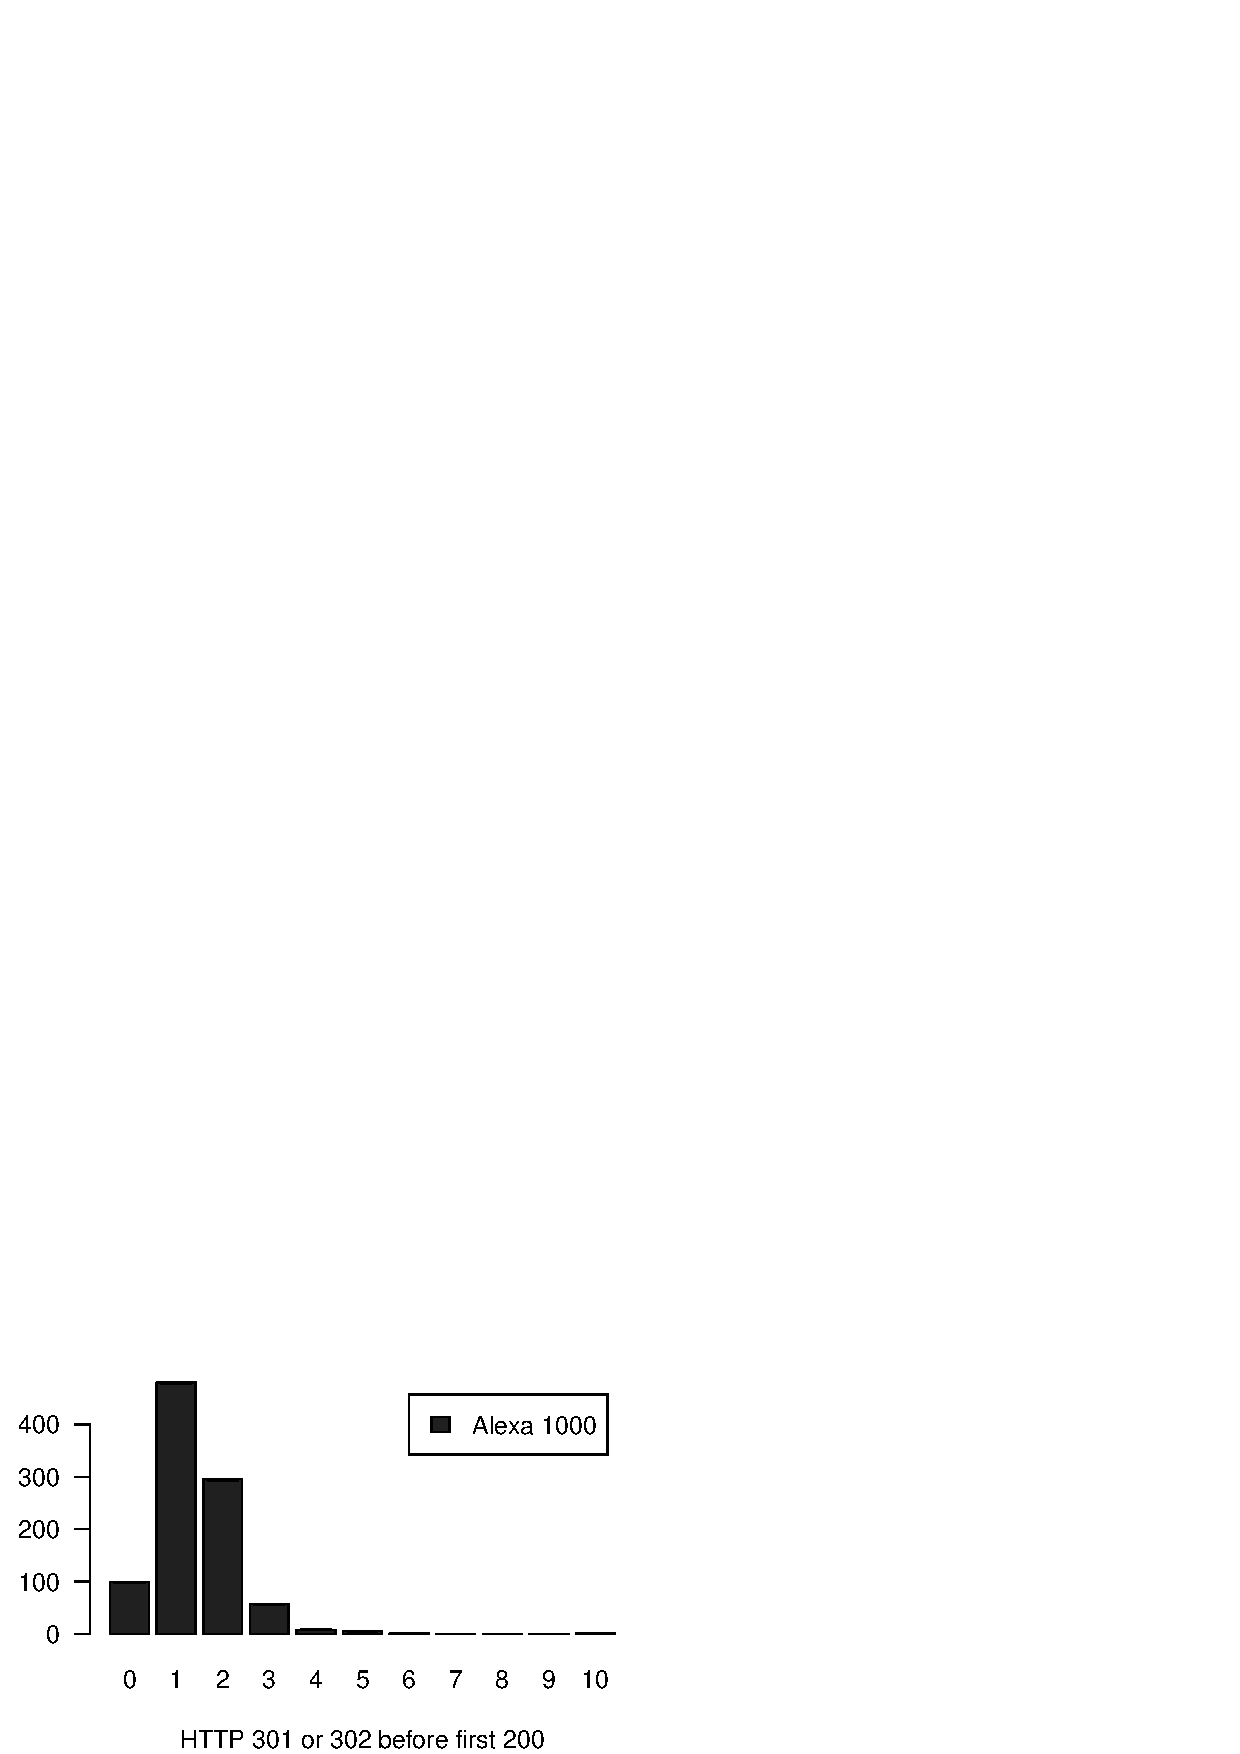
\includegraphics[width=\linewidth]{New_Plots/barplot_redirects_clean.pdf}
	\caption{New Measurements}
	\label{fig:new_bar_redirects}
\end{subfigure}\par\medskip
\begin{subfigure}{\linewidth}
		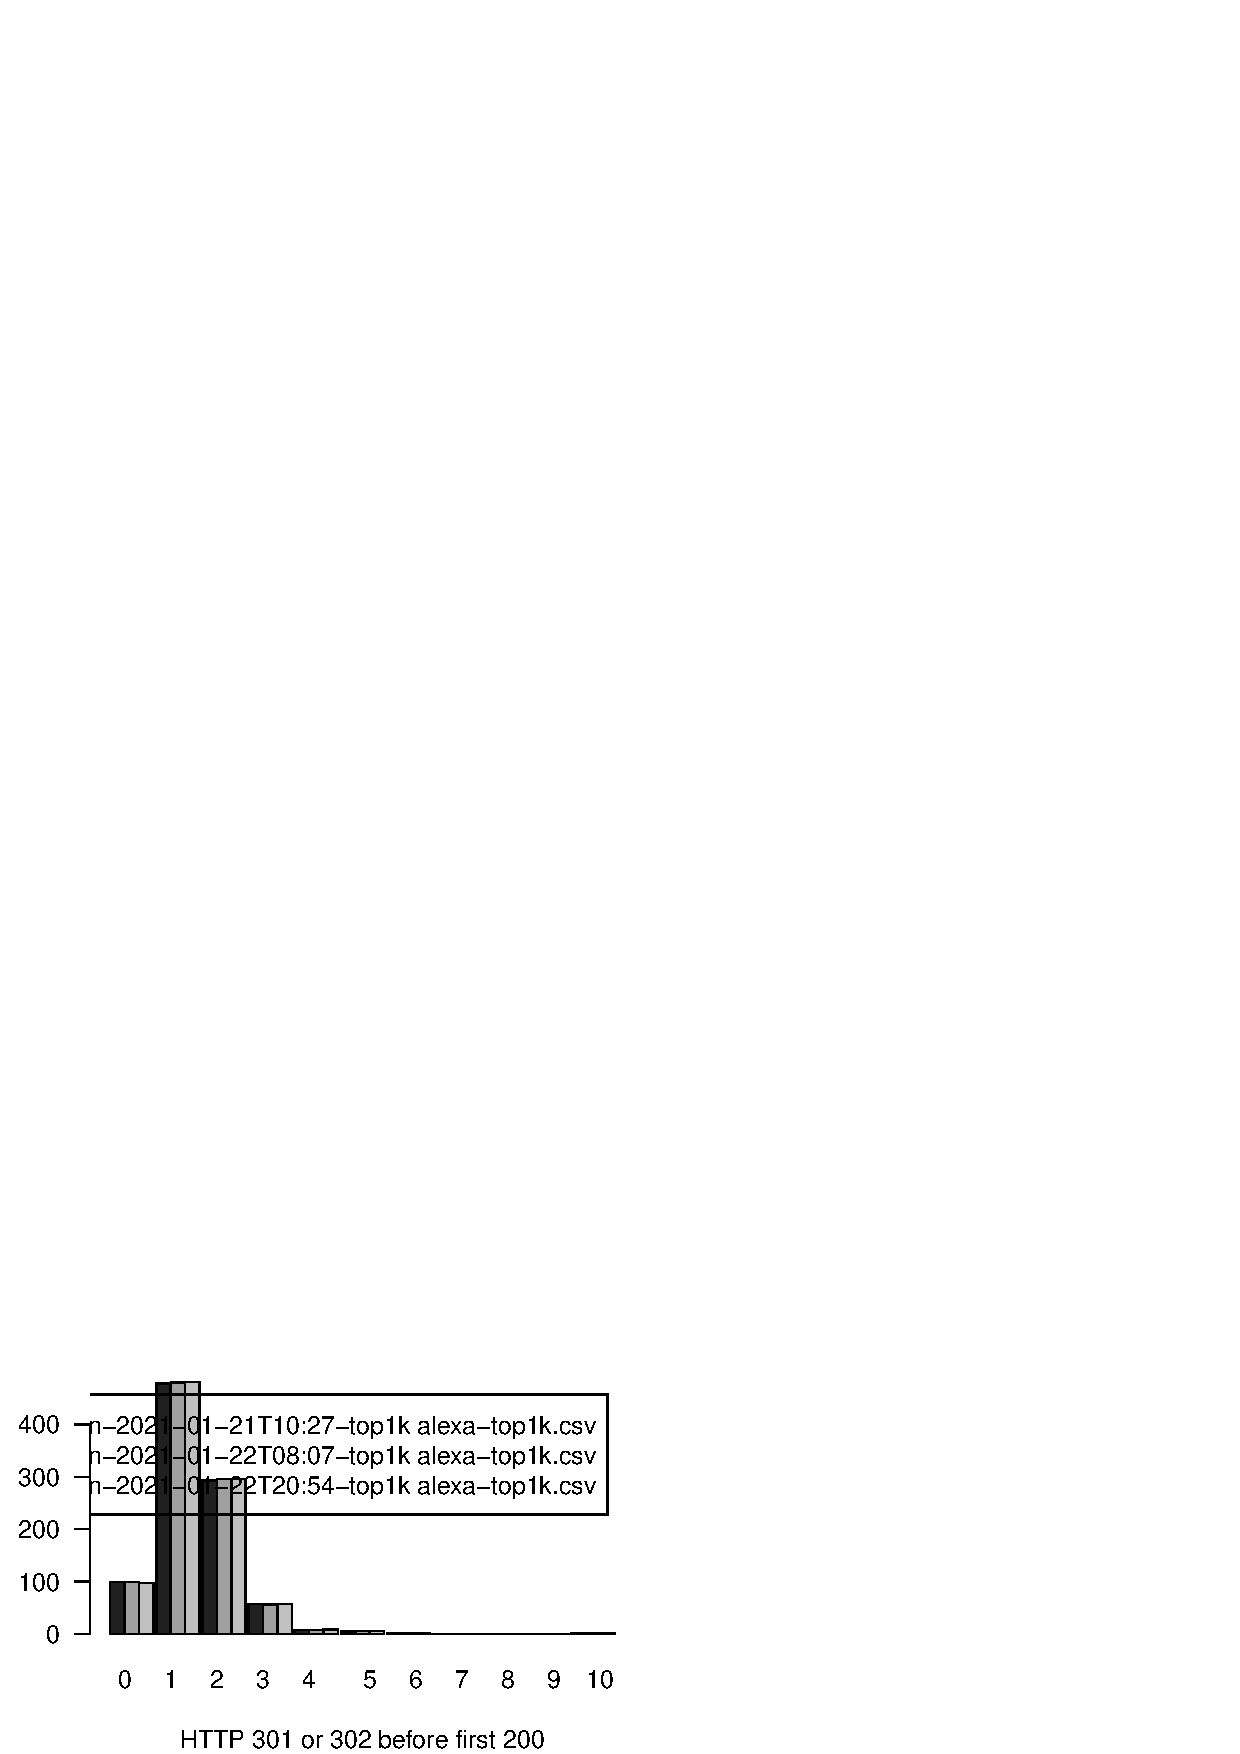
\includegraphics[width=\linewidth]{Original Plots/barplot_redirects.pdf}
	\caption{Original Measurements}
	\label{fig:orig_bar_redirects}
\end{subfigure}
\caption{Number of initial Redirects}
\label{fig:bar_redirects}
\end{figure}

\begin{figure}
 \centering
 \begin{subfigure}{\linewidth}
		\includegraphics[width=\linewidth]{New_Plots/ecdf_loadtimes.pdf}
	\caption{New Measurements}
	\label{fig:new_plot_redirects}
\end{subfigure}\par\medskip
\begin{subfigure}{\linewidth}
		\includegraphics[width=\linewidth]{Original Plots/ecdf_loadtimes.pdf}
	\caption{Original Measurements}
	\label{fig:orig_plot_redirects}
\end{subfigure}
\caption{Page Load Time (PLT) with and without initial redirects}
\label{fig:plot_redirects}
\end{figure}

\subsection{Number and Size of Objects}
In order to estimate the complexity of web pages, metrics such as Object Index, Object Count, and Byte Index are employed. Since web pages are often constantly loading - even after the initial page load - object counts should only count objects loaded by the onLoad event. Calculating a count of the initial objects can be done using objects in the DOM or HTTP request-response pairs. Object size normally reflects the encoded size (i.e. the count of bytes transferred over the network) but can also reflect the decoded (i.e. decompressed) number of bytes. Byte Index refers to the integral of the total sizes of objects loaded over time and is an important metric for the size of Objects \cite{10.1145/2940136.2940138}.

To obtain the number of objects, one can count the number of HTTP request-response pairs in HAR files. The number of objects can also be obtained using the Resource Timings API. Both the Resource Timings API and HAR files supply the encoded and decoded body size. Alternatively, the number of objects can be extracted from packet capture traces if all elements can be decrypted; if this is not the case, object sizes can differ due to TLS padding.
\section{Re-Implementation \& Results}

\begin{frame}
    \frametitle{Re-Implementation Tools}
	\begin{table}
		\centering
		\caption{Comparison Setup \& Tools}
		\label{tab:tools}
		\begin{tabular}{lccccccc}
			\toprule
			& \textbf{Original Paper} & \textbf{Reproduction}\\
			\midrule
			Hardware & Thinkpad L450 & Matebook X Pro (1st Generation)\\
			Operating System & Debian 9 (Stretch) & Ubuntu 20.04\\
			Firefox & 62.0.2 / 61.0.2 & 84.0.2 \\
			Chrome & 69 & 88 \\
			Selenium & 3.14.0 & 3.141.59\\
			Geckodriver & 0.21.0 & 0.29.0\\
			HAR Export Trigger & 0.6.1 & 0.6.1\\
			\bottomrule
		\end{tabular}
	\end{table}
	
Despite trying the versions specified in the original paper as well as the more modern versions, \textbf{it was not possible to consistently extract HAR files using Firefox with Selenium and Chrome with PyDevTools as specified in the original paper}.

$\boldsymbol{\rightarrow}$  This paper focused on reproducing measurements using Firefox with Marionette.
\end{frame}

\begin{frame}
    \frametitle{Results - Redirects}
\begin{figure}
 \centering
 \begin{subfigure}{0.5\textwidth}
 \centering
	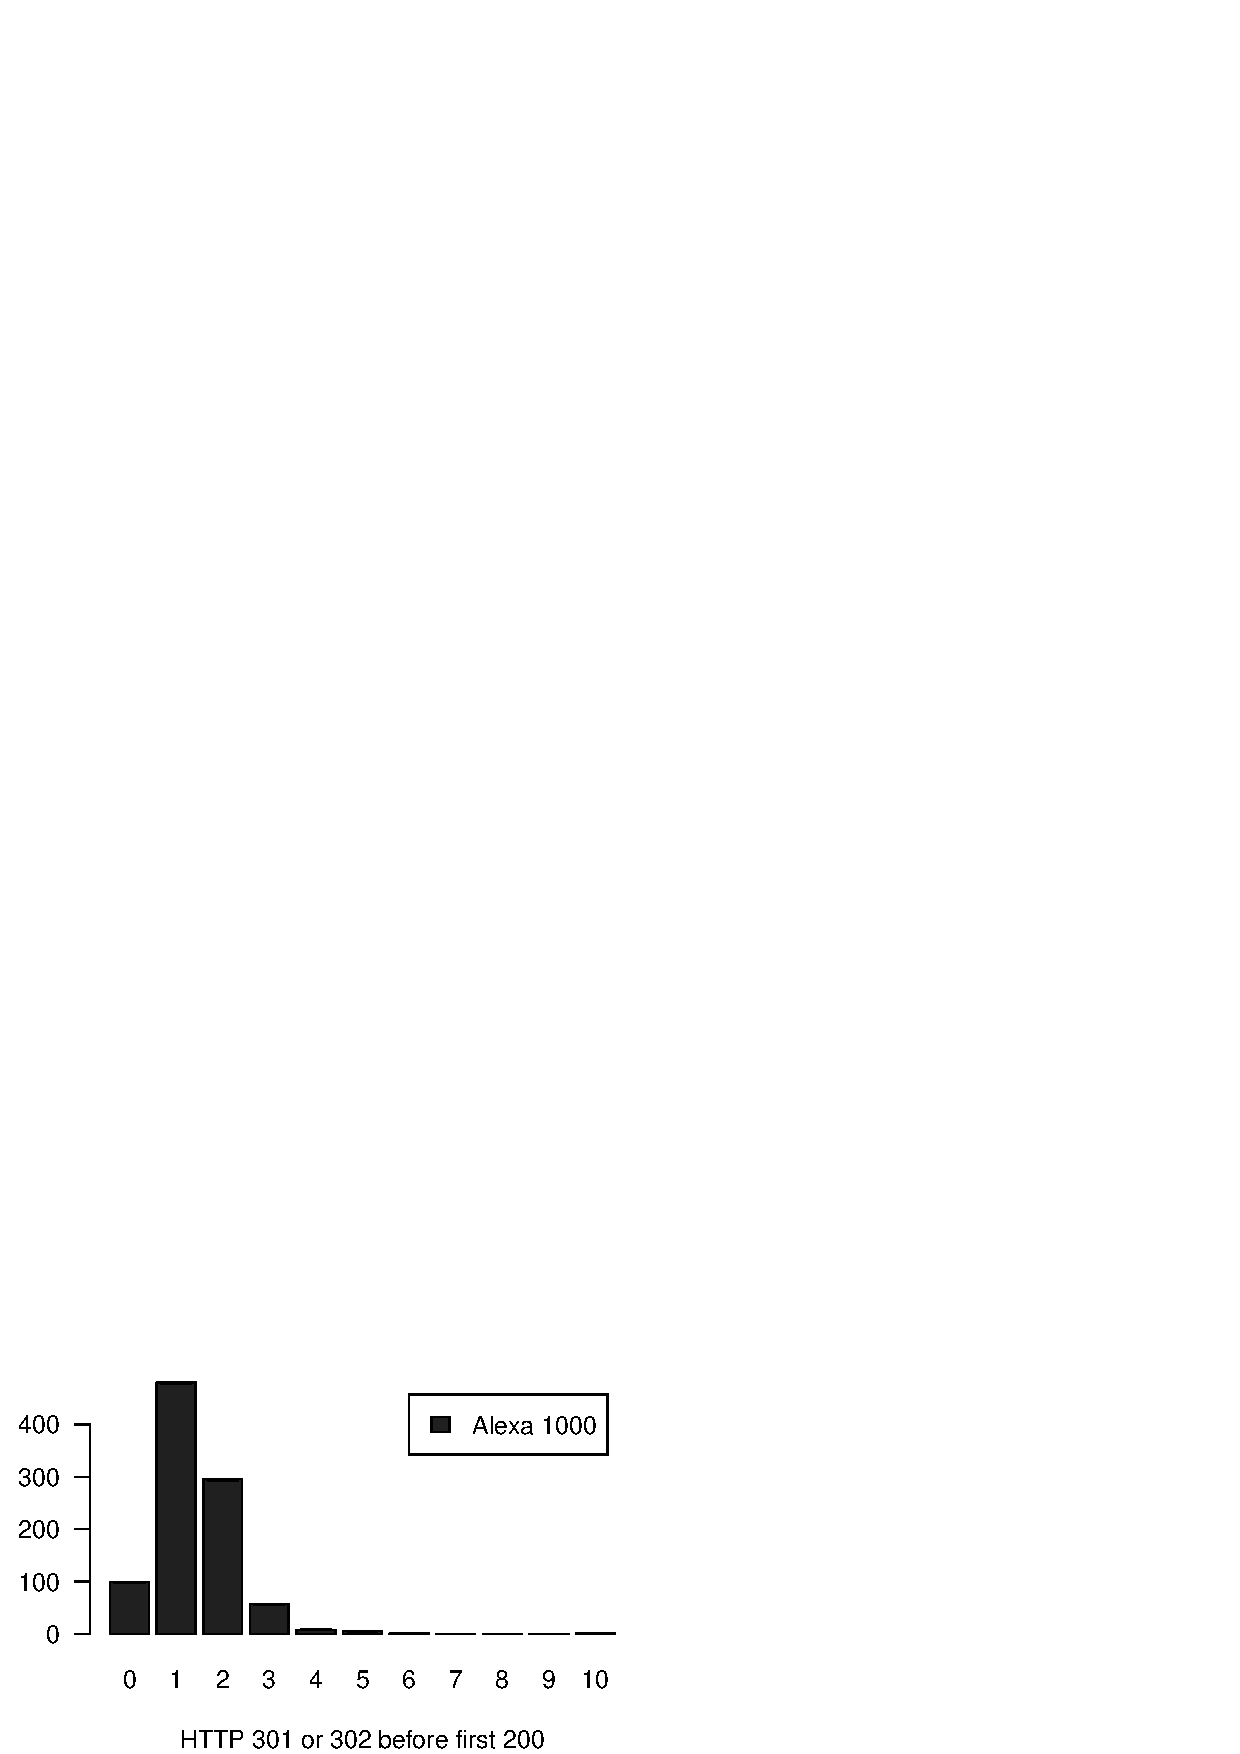
\includegraphics[width=.8\linewidth,keepaspectratio]{New_Plots/barplot_redirects_clean.pdf}
	\caption{New Measurements}
	\label{fig:new_bar_redirects}
	\par\medskip
	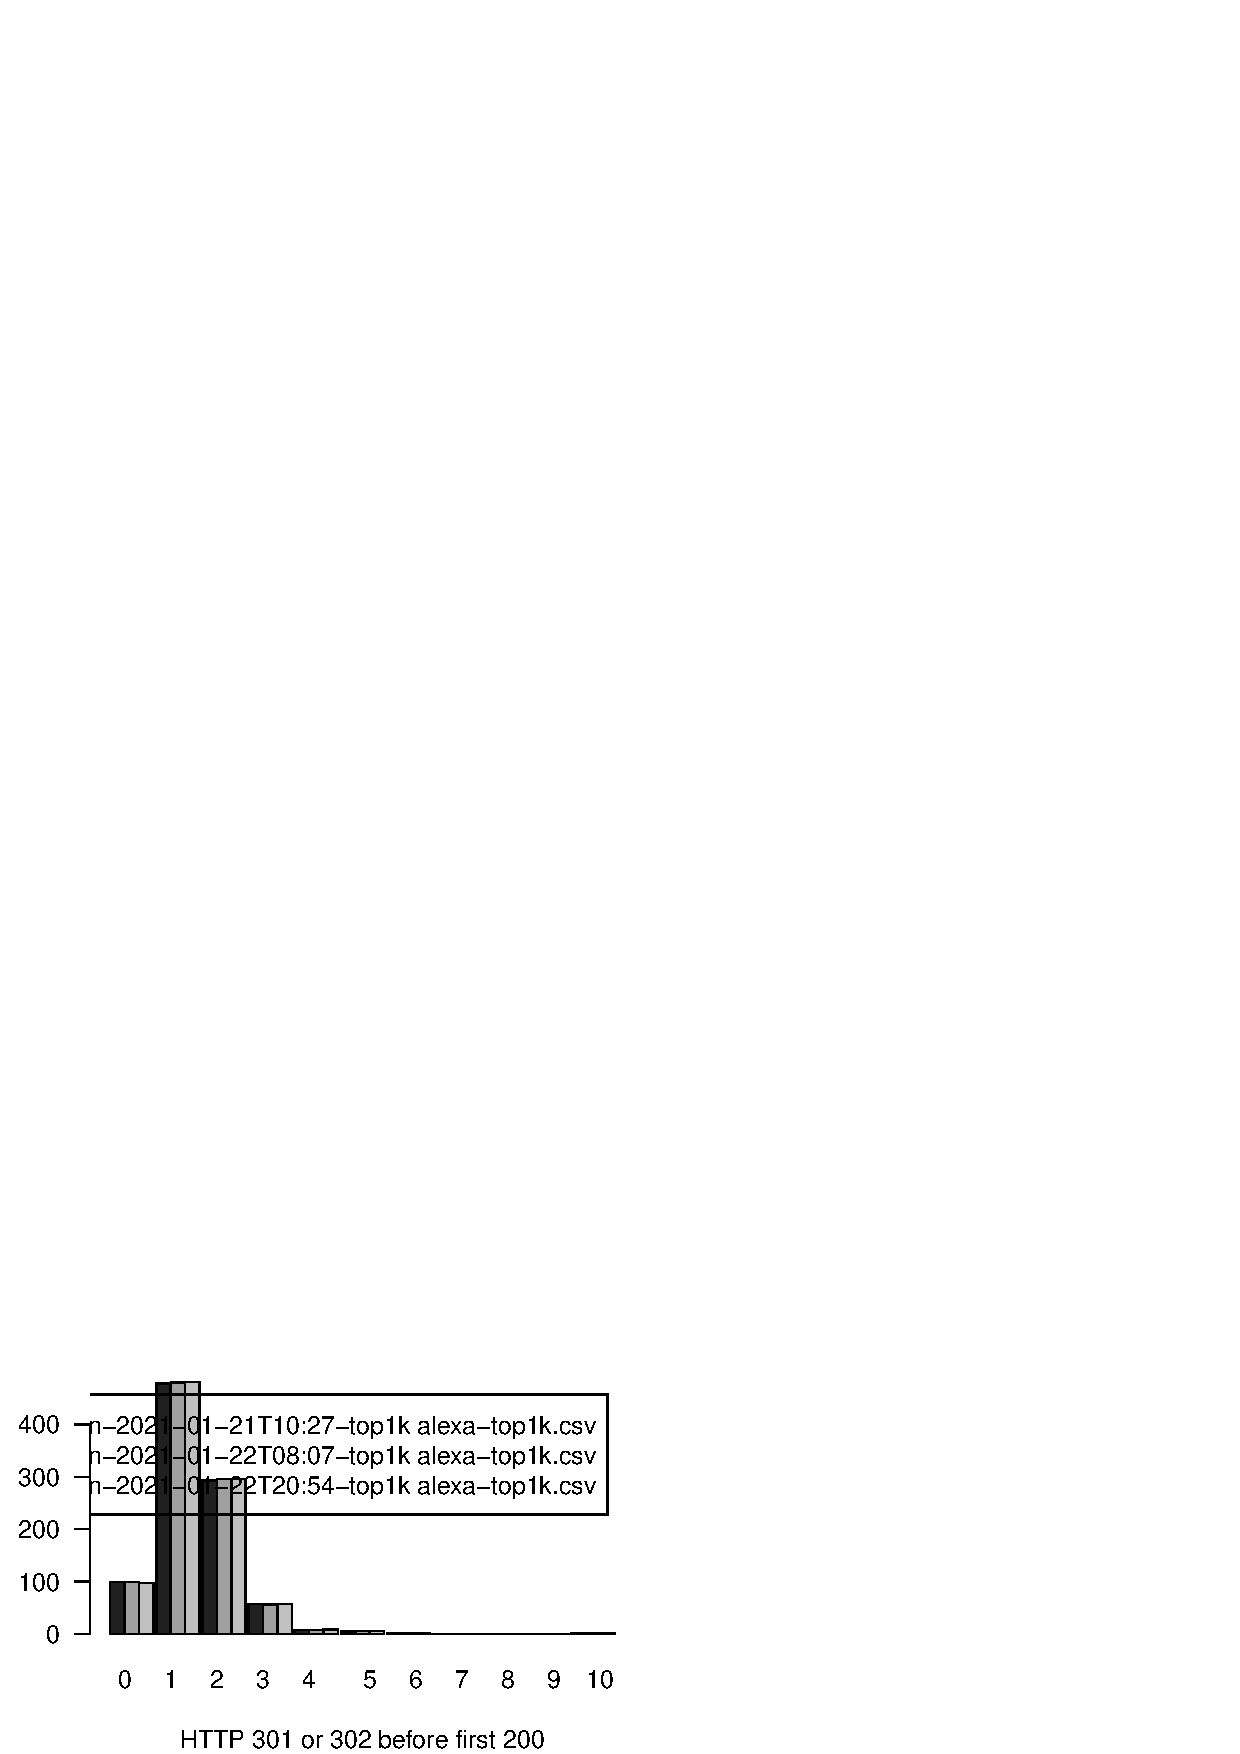
\includegraphics[width=.8\linewidth,keepaspectratio]{Original Plots/barplot_redirects.pdf}
	\caption{Original Measurements}
	\label{fig:orig_bar_redirects}
	\end{subfigure}%
	 \begin{subfigure}{0.5\textwidth}
	 \centering
	\includegraphics[width=.8\linewidth,keepaspectratio]{New_Plots/ecdf_loadtimes.pdf}
	\caption{New Measurements}
	\label{fig:new_plot_redirects}
	\par\medskip
	\includegraphics[width=.8\linewidth,keepaspectratio]{Original Plots/ecdf_loadtimes.pdf}
	\caption{Original Measurements}
	\label{fig:orig_plot_redirects}
	\end{subfigure}
\caption{Number of initial Redirects (Left) \& PLT with and without initial redirects (Right)}
\end{figure}

\end{frame}

\begin{frame}
    \frametitle{Results - Object Sizes}
\begin{figure}
 \centering
 \begin{subfigure}{0.5\textwidth}
 \centering
 	 \includegraphics[width=\linewidth,keepaspectratio]{New_Plots/ecdf_diff_objectsizes.pdf}
	\caption{New Measurements}
	\label{fig:new_absolute_byte_index}
	\end{subfigure}%
	 \begin{subfigure}{0.5\textwidth}
	 \centering
	\includegraphics[width=.8\linewidth,keepaspectratio]{Firefox Plots/ecdf_diff_objectsizes.pdf}
	\caption{Original Measurements (Firefox Only)}
	\label{fig:orig_absolute_byte_index}
	\par\medskip
	\includegraphics[width=.8\linewidth,keepaspectratio]{Chrome_Plots/ecdf_diff_objectsizes.pdf}
	\caption{Original Measurements (Chrome Only)}
	\label{fig:orig_chrome_absolute_byte_index}
	\end{subfigure}
\caption{Object sizes: differences due to metric for all objects}
\end{figure}

\end{frame}


\begin{frame}
    \frametitle{Results - Object Counts / Byte Index}
\begin{figure}
 \centering
 \begin{subfigure}{0.5\textwidth}
 \centering
 	 \includegraphics[width=\linewidth,keepaspectratio]{New_Plots/ecdf_rel_object_byte_index.pdf}
	\caption{New Measurements}
	\label{fig:new_relative_byte_index}

	\end{subfigure}%
	 \begin{subfigure}{0.5\textwidth}
	 \centering
	\includegraphics[width=.8\linewidth,keepaspectratio]{Firefox Plots/ecdf_rel_object_byte_index.pdf}
	\caption{Original Measurements (Firefox Only)}
	\label{fig:orig_firefox_relative_byte_index}
		\par\medskip
		\includegraphics[width=.8\linewidth,keepaspectratio]{Chrome_Plots/ecdf_rel_object_byte_index.pdf}
	\caption{Original Measurements (Chrome Only)}
	\label{fig:orig_chrome_relative_byte_index}
	\end{subfigure}
\caption{Byte index: difference due to data source}
\end{figure}

\end{frame}

\section{Conclusion}

\begin{frame}
    \frametitle{Analysis}
	This reproducibility report shows the following: 
	\begin{itemize}
        \item The new dataset contradicts the conclusion in the original paper that the Content-Length in HAR files is the most reliable data source for object sizes but does confirm the large inconsistencies in object size between data sources.
        \item The other examined conclusions regarding redirects and object count / byte index were confirmed by the new dataset.
        \item The data in both papers underlines the importance of improving the documentation of studies of web performance as well as choosing performance metrics carefully and deliberately. 
   	 \end{itemize}
\end{frame}

\begin{frame}
    \frametitle{Questions?}
      \centering \Large
  	\emph{Thank you for your attention!}
  	
  	Please feel free to ask questions now or contact me after the talk:
    
    \textbf{Curt Polack}
    
    \textbf{curt.polack@tum.de}
    
    
\end{frame}


% Include markdown source from ./pandoc
%\input{pandoc/example}

% Comment out if you do not want a bibliography
\section{Bibliography}
\begin{frame}[allowframebreaks]
    \bibliographystyle{abbrv}
    \setbeamertemplate{bibliography item}[text]
    \footnotesize
    \bibliography{lit}
\end{frame}

\end{document}



\renewcommand{\chairname}{Chair of Connected Mobility}

\begin{document}

% If you are preparing a talk but do not like the default font sizes, you may
% want to try the class option 'beameralt', which uses smaller default font
% sizes and integrates subsection/subsubsection names into the headline.

% For lecture mode, you may want to build one set of slides per chapter but
% with common page numbering. If so,
% 1) create a new .tex file for each chapter, e.g. slides_chapN.tex,
% 2) set the part counter to N-1 (assuming chapters start at 0), and
% 3) and name your chapter by using the \part{} command.
%\setcounter{part}{-1}
%\part{Organisatorisches und Einleitung}

% For 16:9 slides, use the class option 'aspectratio=169'.

% If class option 'noframenumbers' is given, frame numbers are not printed.

% If class option 'notitleframe' is given, the title frame is not autmatically
% generated.

% Class option 'nocontentframes' suppresses automatic generation of content
% frames when new parts/sections are started.

% Include source files from ./include (or ./include/chapN).
\section{Agenda}

\begin{frame}
    \begin{itemize}
        \item Motivation \& Summary of Original Paper
        \item Background: Web Performance Metrics \& Tools
        \item Re-Implementation \& Results
        \item Conclusion
    \end{itemize}
\end{frame}

\section{Motivation \& Summary of Original Paper}

\begin{frame}
    \frametitle{Motivation}
    Web browsing is one of the most widely-used applications used in today's Internet ecosystem. A number of metrics have been developed and used as benchmarks to accurately reflect the performance of web applications for users. \textbf{Measurements can differ greatly depending on a number of factors:}
    \begin{itemize}
        \item Surveyed Web Pages
        \item User Devices
        \item Browsers
        \item Tools (e.g. Selenium)
        \item Metrics
    \end{itemize}
    $\boldsymbol{\rightarrow}$ This diversity as well as the lack of clearly established standards lead to difficulties when quantifying performance. The original paper \cite{10.1007/978-3-030-15986-3_19} examined the effects of these ambiguities with regards to browsers, tools, and metrics and provided guidelines for future papers.
\end{frame}

\begin{frame}
    \frametitle{Summary of Original Paper}
	The original paper \cite{10.1007/978-3-030-15986-3_19} was structured as follows:
    \begin{enumerate}
        \item Introduction
        \item Metric Definitions \& Tools
        \item Survey of 15 Web Studies
        \item Methodology
        \item Identification of Pitfalls \& Guidelines for Future Papers
    \end{enumerate}
\end{frame}
\section{Background}
\label{sec:background}
Among the most important web metrics are load times, number \& size of objects, and page size. Each of the aforementioned metrics can be measured according to numerous definitions and using data from diverse data sources. The following section provides an overview of these definitions and the data sources used in this paper.

\subsection{Load Times}
The time required for loading a web page correlates strongly with user experience \cite{6263888}. A browser normally loads a web page in multiple steps: load and parse the base document, construct a Document Object Model (DOM), load and process referenced objects, render / display the results. Although Page Load Time (PLT), defined as the time until the onLoad event, is most often used to measure page load times, there are a number of other metrics. For example, Time To First Paint (TTFP) and Above The Fold Time (AFT) are triggered before PLT when the content is first displayed and available to the user. The start times used for calculating load times can always differ (e.g. navigationStart, fetchStart). One of the main takeaways from \cite{10.1007/978-3-030-15986-3_19} is that redirects can strongly affect these measurements and should be accounted for; Figure \ref{fig:plot_redirects} shows the impact redirects can have on PLT and Figure \ref{fig:bar_redirects} the prevalence of such redirects. 

There is also a plurality of data sources for calculating load times. The standardized API for navigation timings \cite{timing_2012} is used to fetch load times based on browser events. It is important to note that events / metrics provided by the Navigation Timings API are not necessarily defined in the same way for all browsers. HTTP Archive files \cite{har_format_2012} and the Resource Timings API \cite{w3c_2020} also provide load time data. The majority of modern browsers (e.g. Chrome, Firefox) implement the Navigation Timings and Resource Timings APIs; HAR files can be exported using developer tools. Both Chrome and Firefox provide remote debugging and page load automation interfaces (i.e. Chrome DevTools \& Firefox Marionette). There are also third-party automation frameworks that allow for the same basic functionality as well as extended functions (e.g. keyboard input); Selenium, one of the most popular such tools, is used in the original paper.

 \begin{figure}
 \centering
 \begin{subfigure}{\linewidth}
		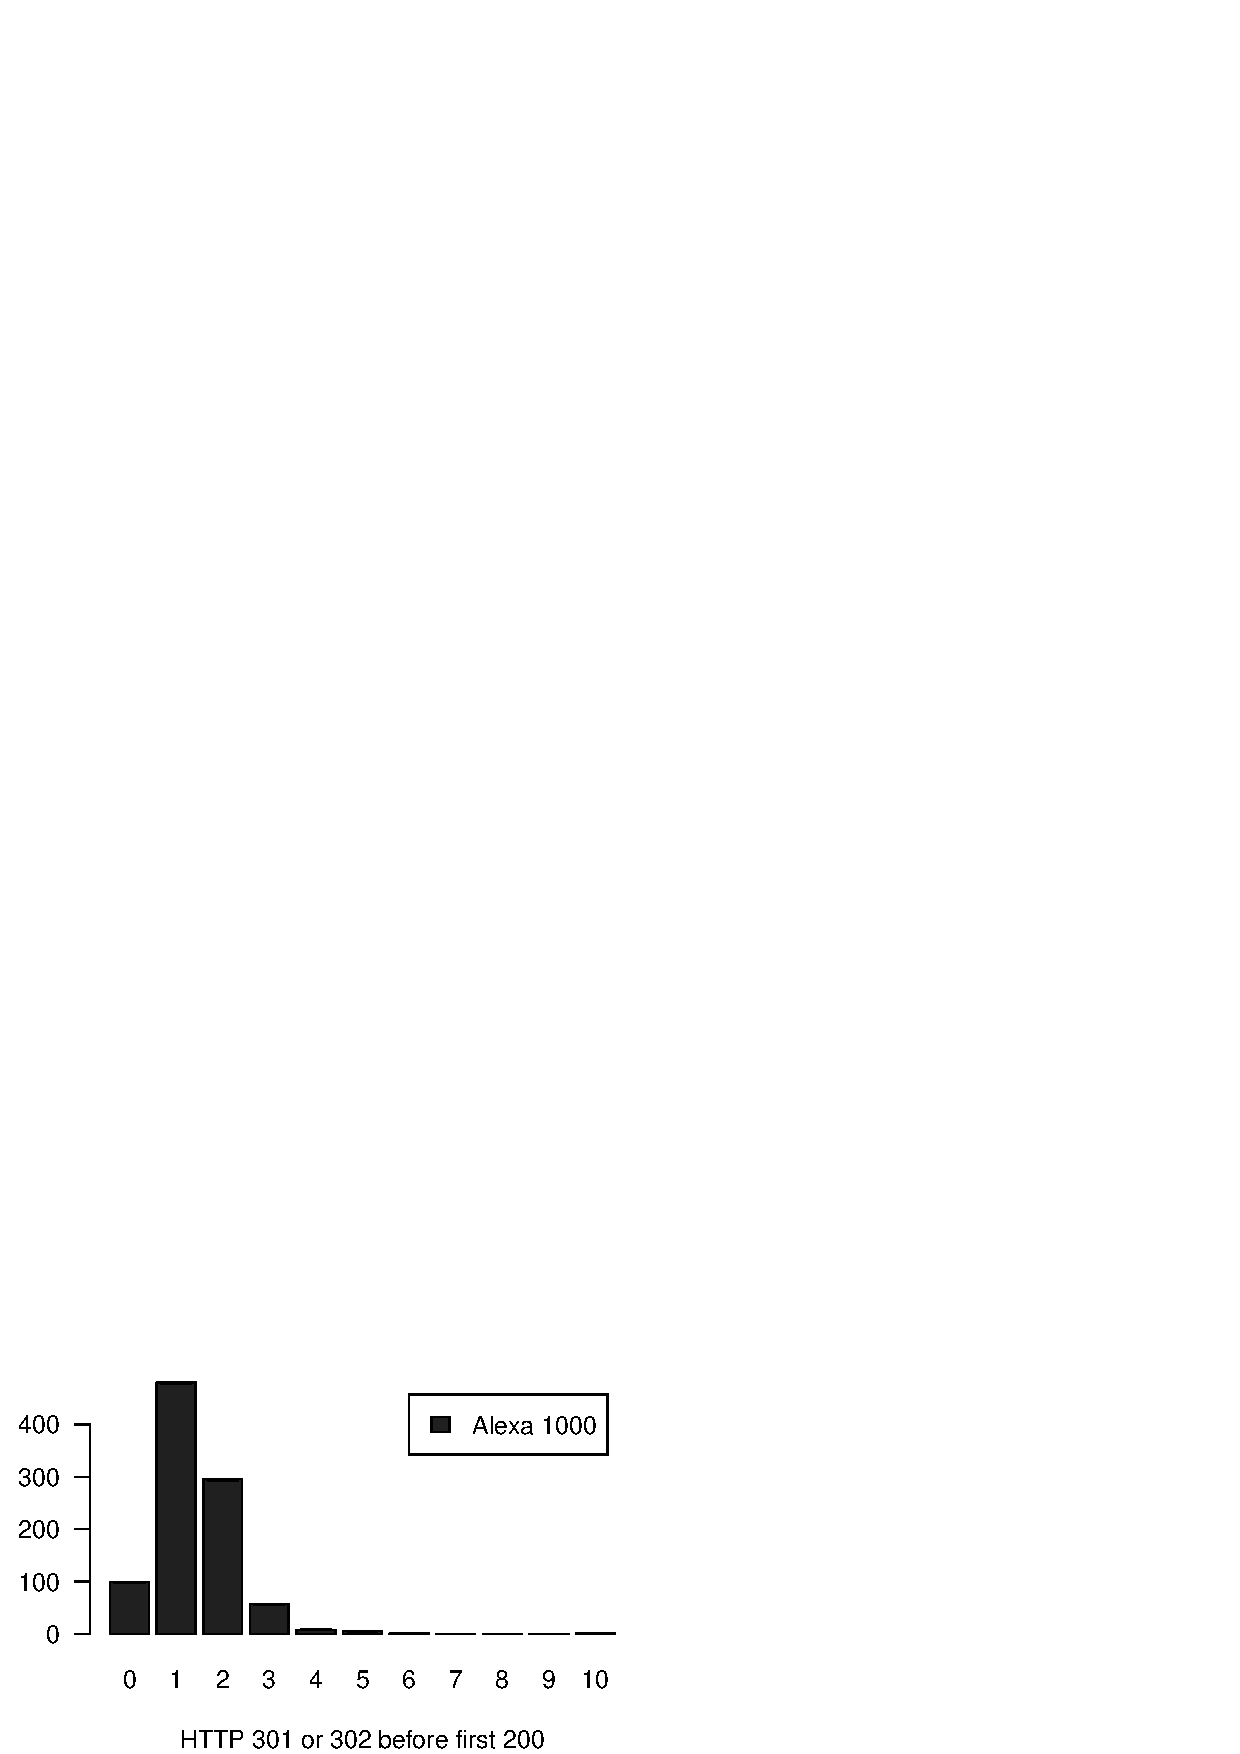
\includegraphics[width=\linewidth]{New_Plots/barplot_redirects_clean.pdf}
	\caption{New Measurements}
	\label{fig:new_bar_redirects}
\end{subfigure}\par\medskip
\begin{subfigure}{\linewidth}
		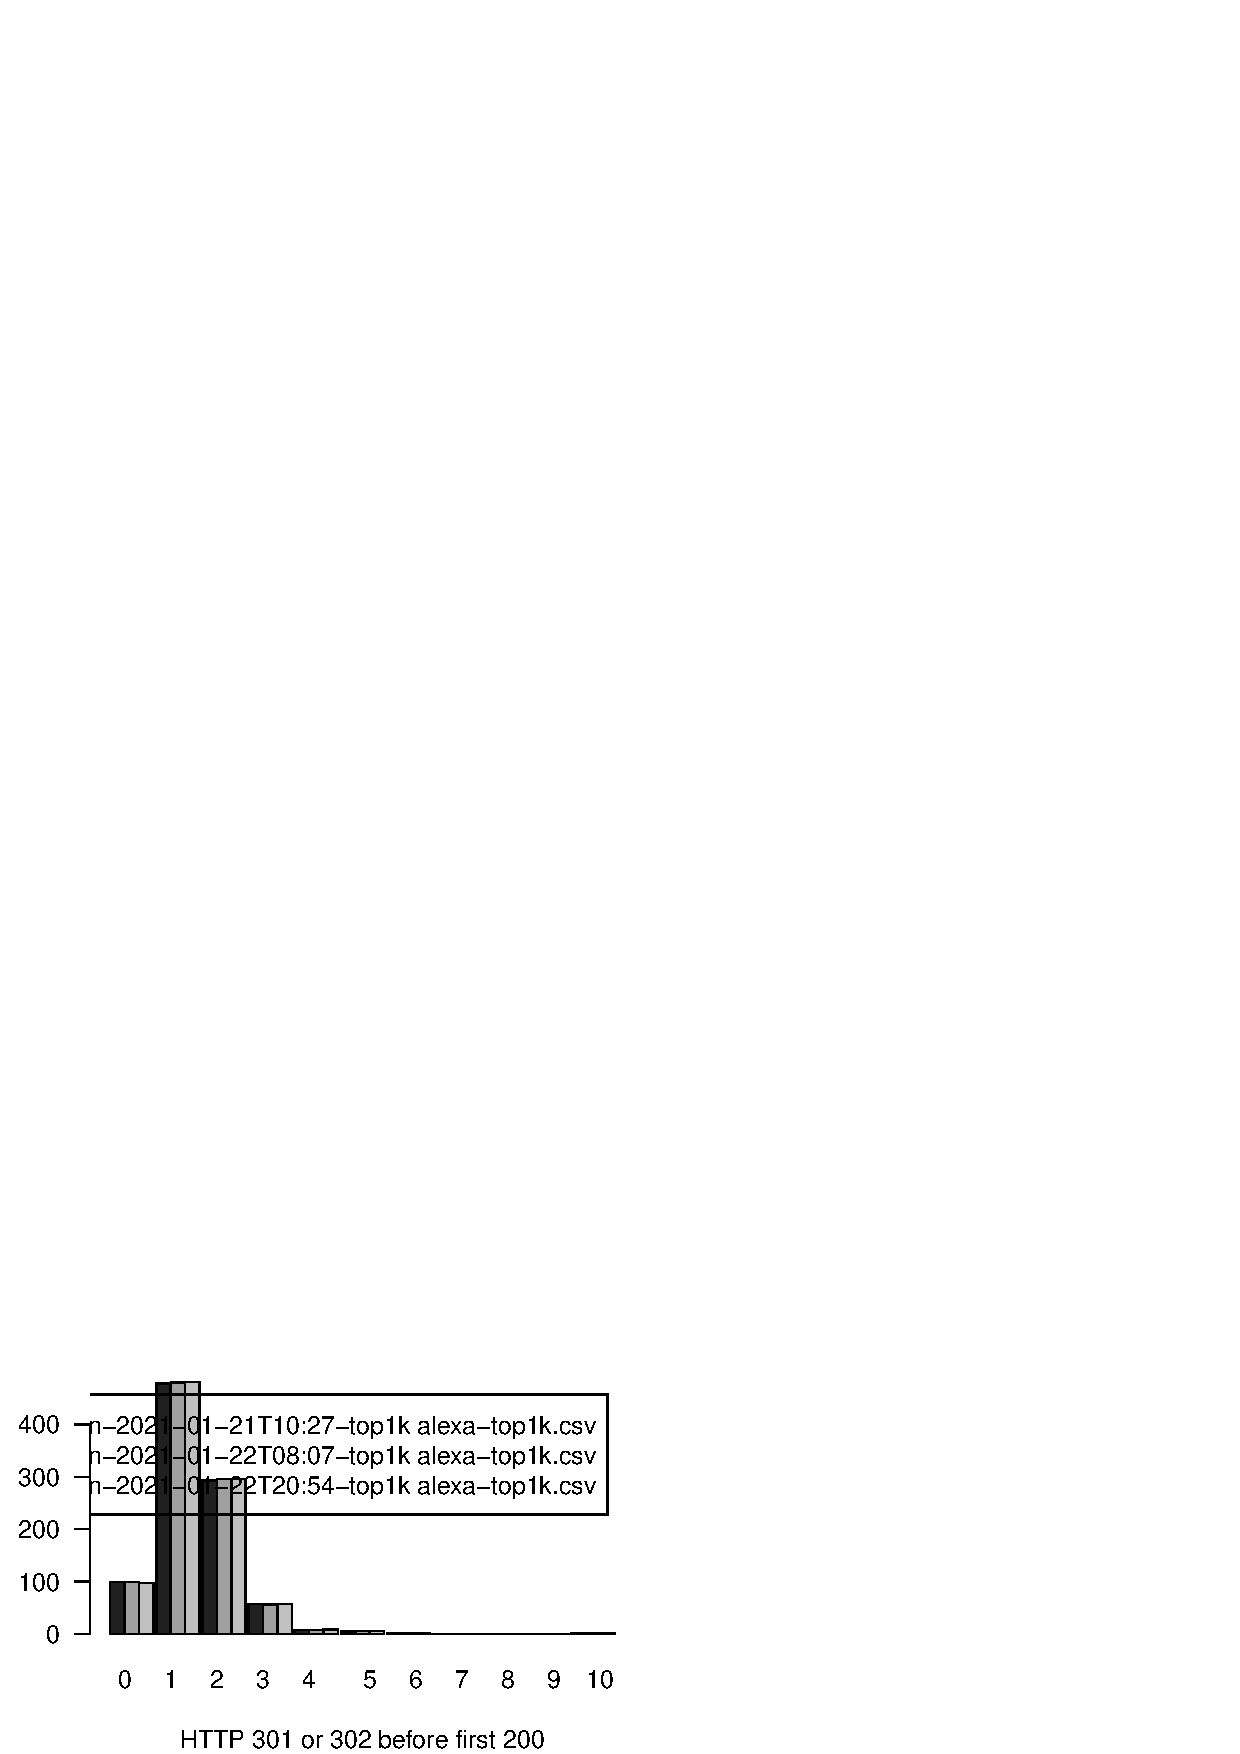
\includegraphics[width=\linewidth]{Original Plots/barplot_redirects.pdf}
	\caption{Original Measurements}
	\label{fig:orig_bar_redirects}
\end{subfigure}
\caption{Number of initial Redirects}
\label{fig:bar_redirects}
\end{figure}

\begin{figure}
 \centering
 \begin{subfigure}{\linewidth}
		\includegraphics[width=\linewidth]{New_Plots/ecdf_loadtimes.pdf}
	\caption{New Measurements}
	\label{fig:new_plot_redirects}
\end{subfigure}\par\medskip
\begin{subfigure}{\linewidth}
		\includegraphics[width=\linewidth]{Original Plots/ecdf_loadtimes.pdf}
	\caption{Original Measurements}
	\label{fig:orig_plot_redirects}
\end{subfigure}
\caption{Page Load Time (PLT) with and without initial redirects}
\label{fig:plot_redirects}
\end{figure}

\subsection{Number and Size of Objects}
In order to estimate the complexity of web pages, metrics such as Object Index, Object Count, and Byte Index are employed. Since web pages are often constantly loading - even after the initial page load - object counts should only count objects loaded by the onLoad event. Calculating a count of the initial objects can be done using objects in the DOM or HTTP request-response pairs. Object size normally reflects the encoded size (i.e. the count of bytes transferred over the network) but can also reflect the decoded (i.e. decompressed) number of bytes. Byte Index refers to the integral of the total sizes of objects loaded over time and is an important metric for the size of Objects \cite{10.1145/2940136.2940138}.

To obtain the number of objects, one can count the number of HTTP request-response pairs in HAR files. The number of objects can also be obtained using the Resource Timings API. Both the Resource Timings API and HAR files supply the encoded and decoded body size. Alternatively, the number of objects can be extracted from packet capture traces if all elements can be decrypted; if this is not the case, object sizes can differ due to TLS padding.
\section{Re-Implementation \& Results}

\begin{frame}
    \frametitle{Re-Implementation Tools}
	\begin{table}
		\centering
		\caption{Comparison Setup \& Tools}
		\label{tab:tools}
		\begin{tabular}{lccccccc}
			\toprule
			& \textbf{Original Paper} & \textbf{Reproduction}\\
			\midrule
			Hardware & Thinkpad L450 & Matebook X Pro (1st Generation)\\
			Operating System & Debian 9 (Stretch) & Ubuntu 20.04\\
			Firefox & 62.0.2 / 61.0.2 & 84.0.2 \\
			Chrome & 69 & 88 \\
			Selenium & 3.14.0 & 3.141.59\\
			Geckodriver & 0.21.0 & 0.29.0\\
			HAR Export Trigger & 0.6.1 & 0.6.1\\
			\bottomrule
		\end{tabular}
	\end{table}
	
Despite trying the versions specified in the original paper as well as the more modern versions, \textbf{it was not possible to consistently extract HAR files using Firefox with Selenium and Chrome with PyDevTools as specified in the original paper}.

$\boldsymbol{\rightarrow}$  This paper focused on reproducing measurements using Firefox with Marionette.
\end{frame}

\begin{frame}
    \frametitle{Results - Redirects}
\begin{figure}
 \centering
 \begin{subfigure}{0.5\textwidth}
 \centering
	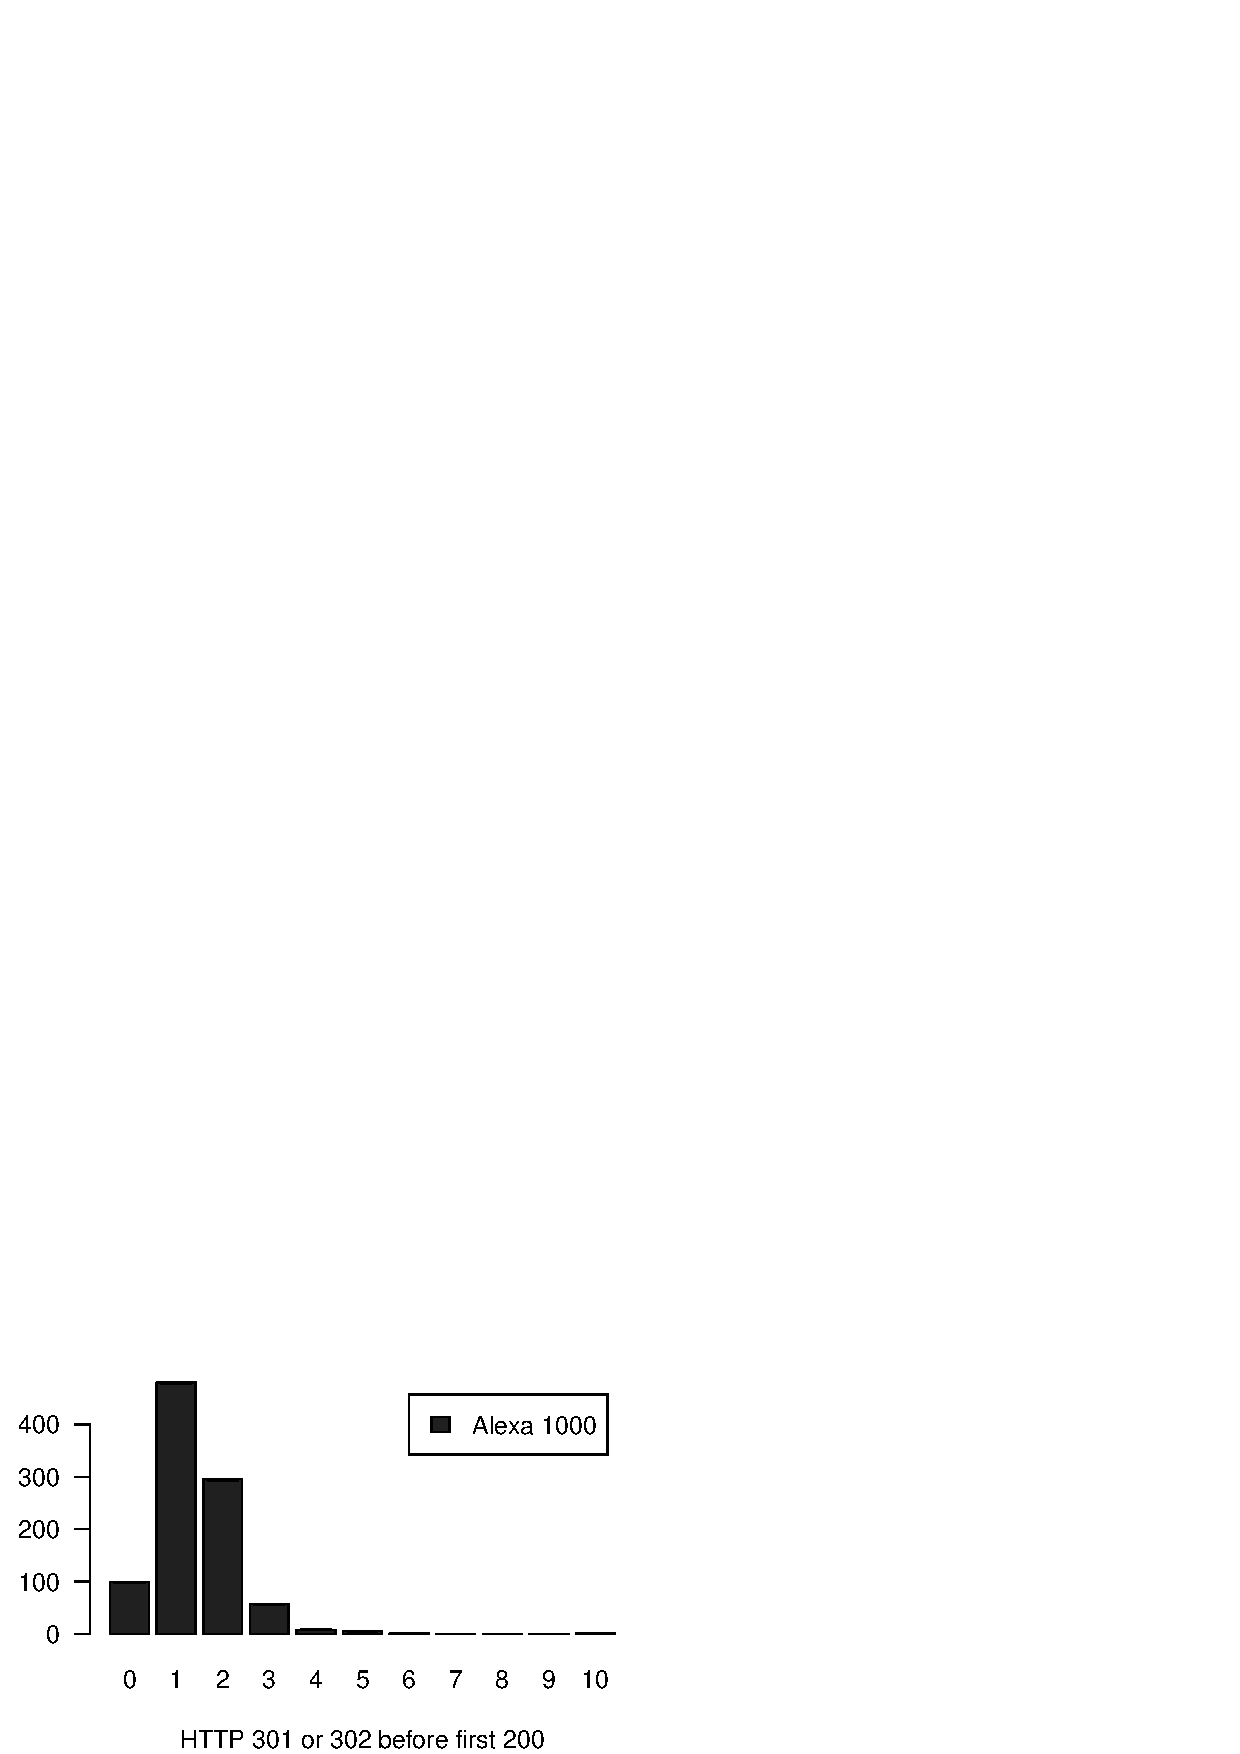
\includegraphics[width=.8\linewidth,keepaspectratio]{New_Plots/barplot_redirects_clean.pdf}
	\caption{New Measurements}
	\label{fig:new_bar_redirects}
	\par\medskip
	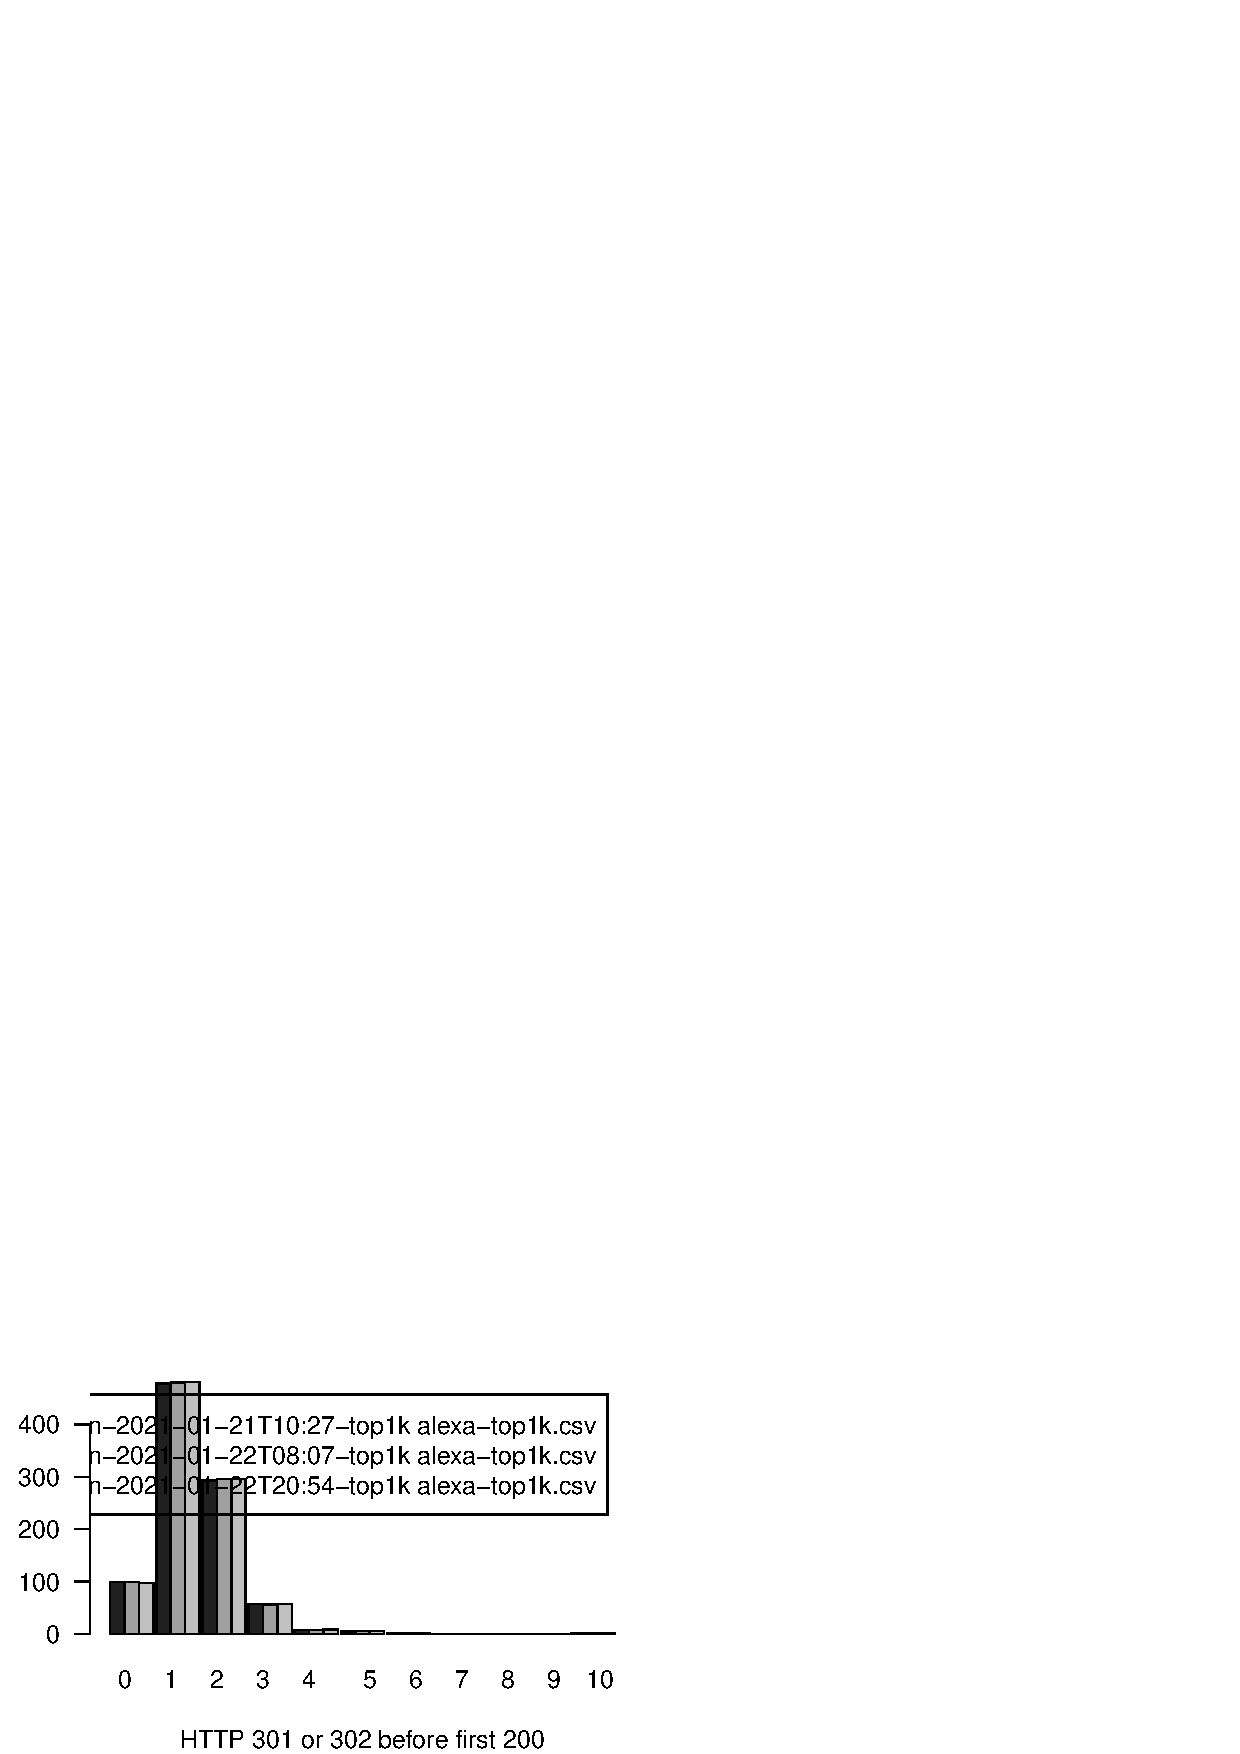
\includegraphics[width=.8\linewidth,keepaspectratio]{Original Plots/barplot_redirects.pdf}
	\caption{Original Measurements}
	\label{fig:orig_bar_redirects}
	\end{subfigure}%
	 \begin{subfigure}{0.5\textwidth}
	 \centering
	\includegraphics[width=.8\linewidth,keepaspectratio]{New_Plots/ecdf_loadtimes.pdf}
	\caption{New Measurements}
	\label{fig:new_plot_redirects}
	\par\medskip
	\includegraphics[width=.8\linewidth,keepaspectratio]{Original Plots/ecdf_loadtimes.pdf}
	\caption{Original Measurements}
	\label{fig:orig_plot_redirects}
	\end{subfigure}
\caption{Number of initial Redirects (Left) \& PLT with and without initial redirects (Right)}
\end{figure}

\end{frame}

\begin{frame}
    \frametitle{Results - Object Sizes}
\begin{figure}
 \centering
 \begin{subfigure}{0.5\textwidth}
 \centering
 	 \includegraphics[width=\linewidth,keepaspectratio]{New_Plots/ecdf_diff_objectsizes.pdf}
	\caption{New Measurements}
	\label{fig:new_absolute_byte_index}
	\end{subfigure}%
	 \begin{subfigure}{0.5\textwidth}
	 \centering
	\includegraphics[width=.8\linewidth,keepaspectratio]{Firefox Plots/ecdf_diff_objectsizes.pdf}
	\caption{Original Measurements (Firefox Only)}
	\label{fig:orig_absolute_byte_index}
	\par\medskip
	\includegraphics[width=.8\linewidth,keepaspectratio]{Chrome_Plots/ecdf_diff_objectsizes.pdf}
	\caption{Original Measurements (Chrome Only)}
	\label{fig:orig_chrome_absolute_byte_index}
	\end{subfigure}
\caption{Object sizes: differences due to metric for all objects}
\end{figure}

\end{frame}


\begin{frame}
    \frametitle{Results - Object Counts / Byte Index}
\begin{figure}
 \centering
 \begin{subfigure}{0.5\textwidth}
 \centering
 	 \includegraphics[width=\linewidth,keepaspectratio]{New_Plots/ecdf_rel_object_byte_index.pdf}
	\caption{New Measurements}
	\label{fig:new_relative_byte_index}

	\end{subfigure}%
	 \begin{subfigure}{0.5\textwidth}
	 \centering
	\includegraphics[width=.8\linewidth,keepaspectratio]{Firefox Plots/ecdf_rel_object_byte_index.pdf}
	\caption{Original Measurements (Firefox Only)}
	\label{fig:orig_firefox_relative_byte_index}
		\par\medskip
		\includegraphics[width=.8\linewidth,keepaspectratio]{Chrome_Plots/ecdf_rel_object_byte_index.pdf}
	\caption{Original Measurements (Chrome Only)}
	\label{fig:orig_chrome_relative_byte_index}
	\end{subfigure}
\caption{Byte index: difference due to data source}
\end{figure}

\end{frame}

\section{Conclusion}

\begin{frame}
    \frametitle{Analysis}
	This reproducibility report shows the following: 
	\begin{itemize}
        \item The new dataset contradicts the conclusion in the original paper that the Content-Length in HAR files is the most reliable data source for object sizes but does confirm the large inconsistencies in object size between data sources.
        \item The other examined conclusions regarding redirects and object count / byte index were confirmed by the new dataset.
        \item The data in both papers underlines the importance of improving the documentation of studies of web performance as well as choosing performance metrics carefully and deliberately. 
   	 \end{itemize}
\end{frame}

\begin{frame}
    \frametitle{Questions?}
      \centering \Large
  	\emph{Thank you for your attention!}
  	
  	Please feel free to ask questions now or contact me after the talk:
    
    \textbf{Curt Polack}
    
    \textbf{curt.polack@tum.de}
    
    
\end{frame}


% Include markdown source from ./pandoc
%\input{pandoc/example}

% Comment out if you do not want a bibliography
\section{Bibliography}
\begin{frame}[allowframebreaks]
    \bibliographystyle{abbrv}
    \setbeamertemplate{bibliography item}[text]
    \footnotesize
    \bibliography{lit}
\end{frame}

\end{document}



\renewcommand{\chairname}{Chair of Connected Mobility}

\begin{document}

% If you are preparing a talk but do not like the default font sizes, you may
% want to try the class option 'beameralt', which uses smaller default font
% sizes and integrates subsection/subsubsection names into the headline.

% For lecture mode, you may want to build one set of slides per chapter but
% with common page numbering. If so,
% 1) create a new .tex file for each chapter, e.g. slides_chapN.tex,
% 2) set the part counter to N-1 (assuming chapters start at 0), and
% 3) and name your chapter by using the \part{} command.
%\setcounter{part}{-1}
%\part{Organisatorisches und Einleitung}

% For 16:9 slides, use the class option 'aspectratio=169'.

% If class option 'noframenumbers' is given, frame numbers are not printed.

% If class option 'notitleframe' is given, the title frame is not autmatically
% generated.

% Class option 'nocontentframes' suppresses automatic generation of content
% frames when new parts/sections are started.

% Include source files from ./include (or ./include/chapN).
\section{Agenda}

\begin{frame}
    \begin{itemize}
        \item Motivation \& Summary of Original Paper
        \item Background: Web Performance Metrics \& Tools
        \item Re-Implementation \& Results
        \item Conclusion
    \end{itemize}
\end{frame}

\section{Motivation \& Summary of Original Paper}

\begin{frame}
    \frametitle{Motivation}
    Web browsing is one of the most widely-used applications used in today's Internet ecosystem. A number of metrics have been developed and used as benchmarks to accurately reflect the performance of web applications for users. \textbf{Measurements can differ greatly depending on a number of factors:}
    \begin{itemize}
        \item Surveyed Web Pages
        \item User Devices
        \item Browsers
        \item Tools (e.g. Selenium)
        \item Metrics
    \end{itemize}
    $\boldsymbol{\rightarrow}$ This diversity as well as the lack of clearly established standards lead to difficulties when quantifying performance. The original paper \cite{10.1007/978-3-030-15986-3_19} examined the effects of these ambiguities with regards to browsers, tools, and metrics and provided guidelines for future papers.
\end{frame}

\begin{frame}
    \frametitle{Summary of Original Paper}
	The original paper \cite{10.1007/978-3-030-15986-3_19} was structured as follows:
    \begin{enumerate}
        \item Introduction
        \item Metric Definitions \& Tools
        \item Survey of 15 Web Studies
        \item Methodology
        \item Identification of Pitfalls \& Guidelines for Future Papers
    \end{enumerate}
\end{frame}
\section{Background}
\label{sec:background}
Among the most important web metrics are load times, number \& size of objects, and page size. Each of the aforementioned metrics can be measured according to numerous definitions and using data from diverse data sources. The following section provides an overview of these definitions and the data sources used in this paper.

\subsection{Load Times}
The time required for loading a web page correlates strongly with user experience \cite{6263888}. A browser normally loads a web page in multiple steps: load and parse the base document, construct a Document Object Model (DOM), load and process referenced objects, render / display the results. Although Page Load Time (PLT), defined as the time until the onLoad event, is most often used to measure page load times, there are a number of other metrics. For example, Time To First Paint (TTFP) and Above The Fold Time (AFT) are triggered before PLT when the content is first displayed and available to the user. The start times used for calculating load times can always differ (e.g. navigationStart, fetchStart). One of the main takeaways from \cite{10.1007/978-3-030-15986-3_19} is that redirects can strongly affect these measurements and should be accounted for; Figure \ref{fig:plot_redirects} shows the impact redirects can have on PLT and Figure \ref{fig:bar_redirects} the prevalence of such redirects. 

There is also a plurality of data sources for calculating load times. The standardized API for navigation timings \cite{timing_2012} is used to fetch load times based on browser events. It is important to note that events / metrics provided by the Navigation Timings API are not necessarily defined in the same way for all browsers. HTTP Archive files \cite{har_format_2012} and the Resource Timings API \cite{w3c_2020} also provide load time data. The majority of modern browsers (e.g. Chrome, Firefox) implement the Navigation Timings and Resource Timings APIs; HAR files can be exported using developer tools. Both Chrome and Firefox provide remote debugging and page load automation interfaces (i.e. Chrome DevTools \& Firefox Marionette). There are also third-party automation frameworks that allow for the same basic functionality as well as extended functions (e.g. keyboard input); Selenium, one of the most popular such tools, is used in the original paper.

 \begin{figure}
 \centering
 \begin{subfigure}{\linewidth}
		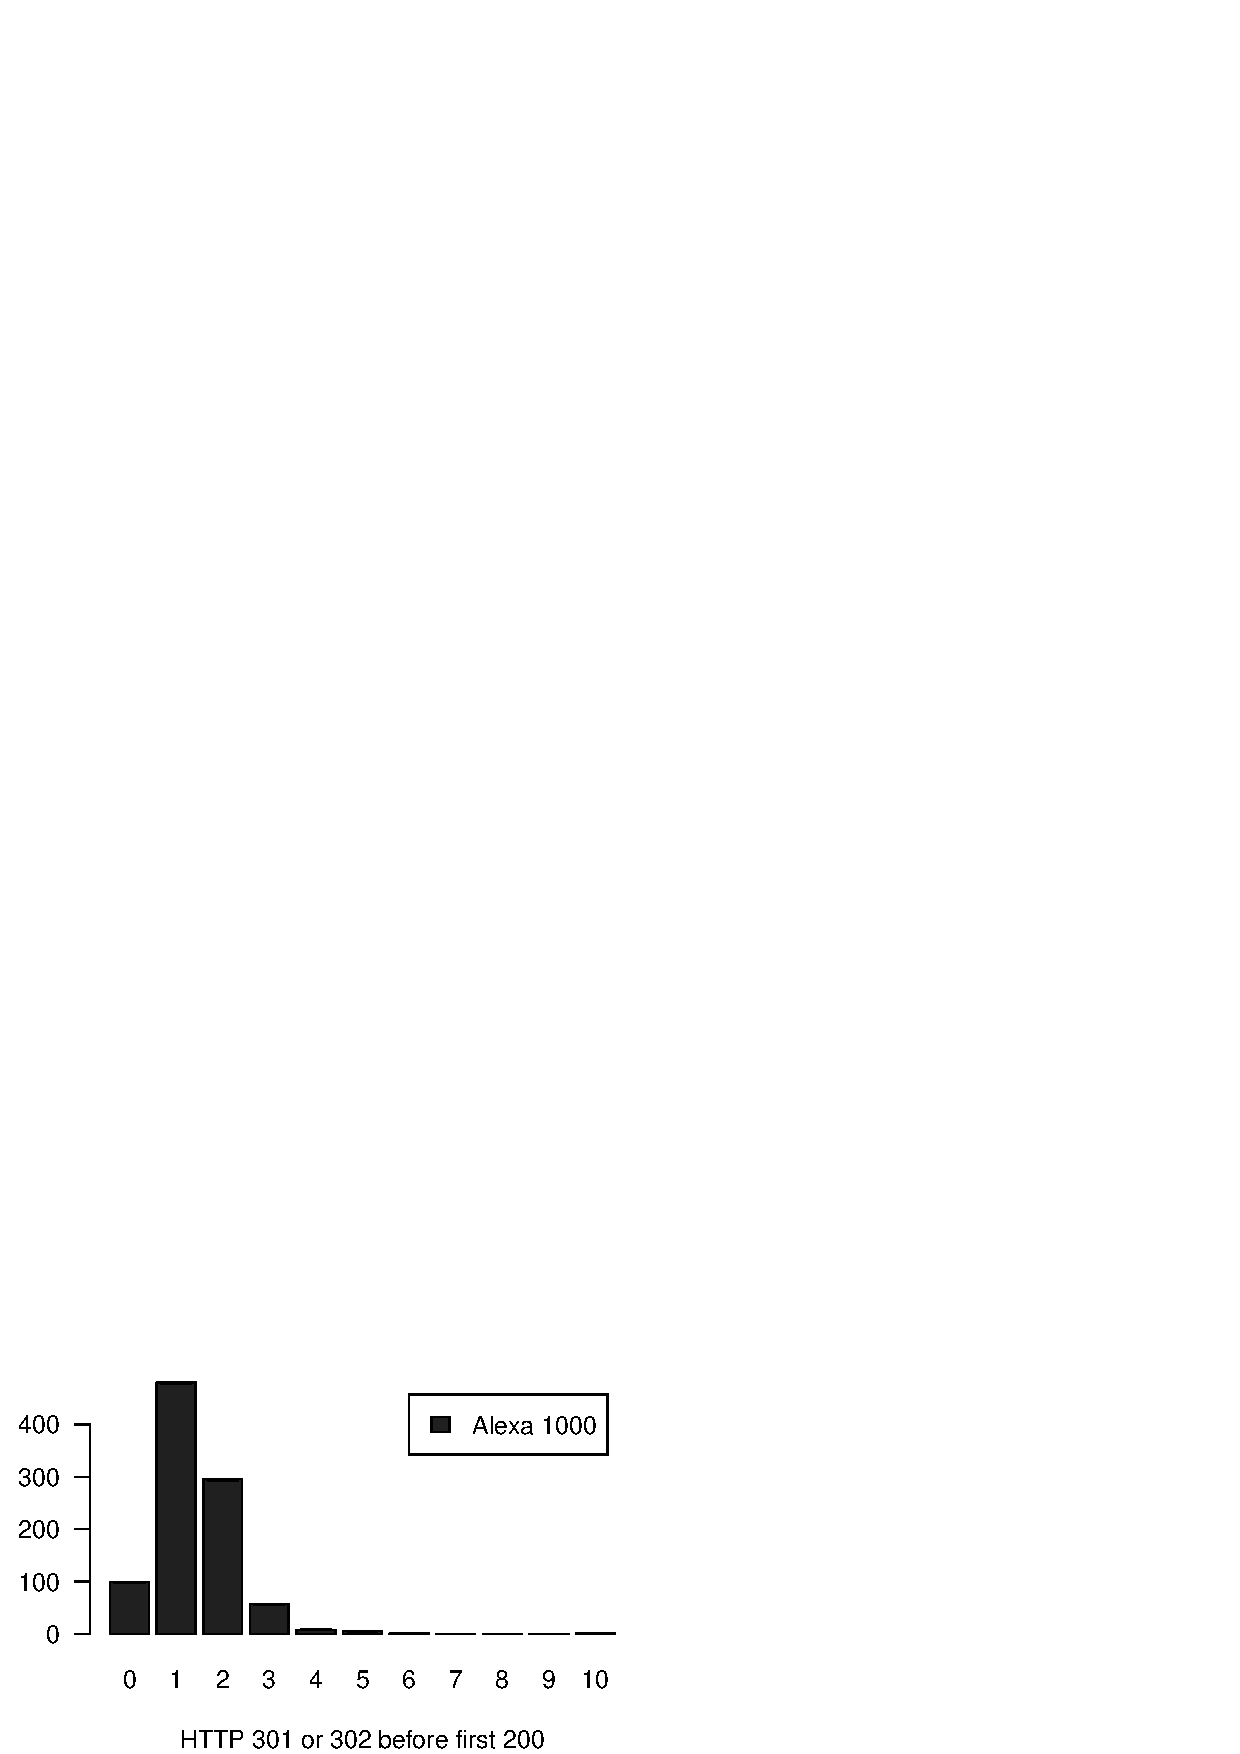
\includegraphics[width=\linewidth]{New_Plots/barplot_redirects_clean.pdf}
	\caption{New Measurements}
	\label{fig:new_bar_redirects}
\end{subfigure}\par\medskip
\begin{subfigure}{\linewidth}
		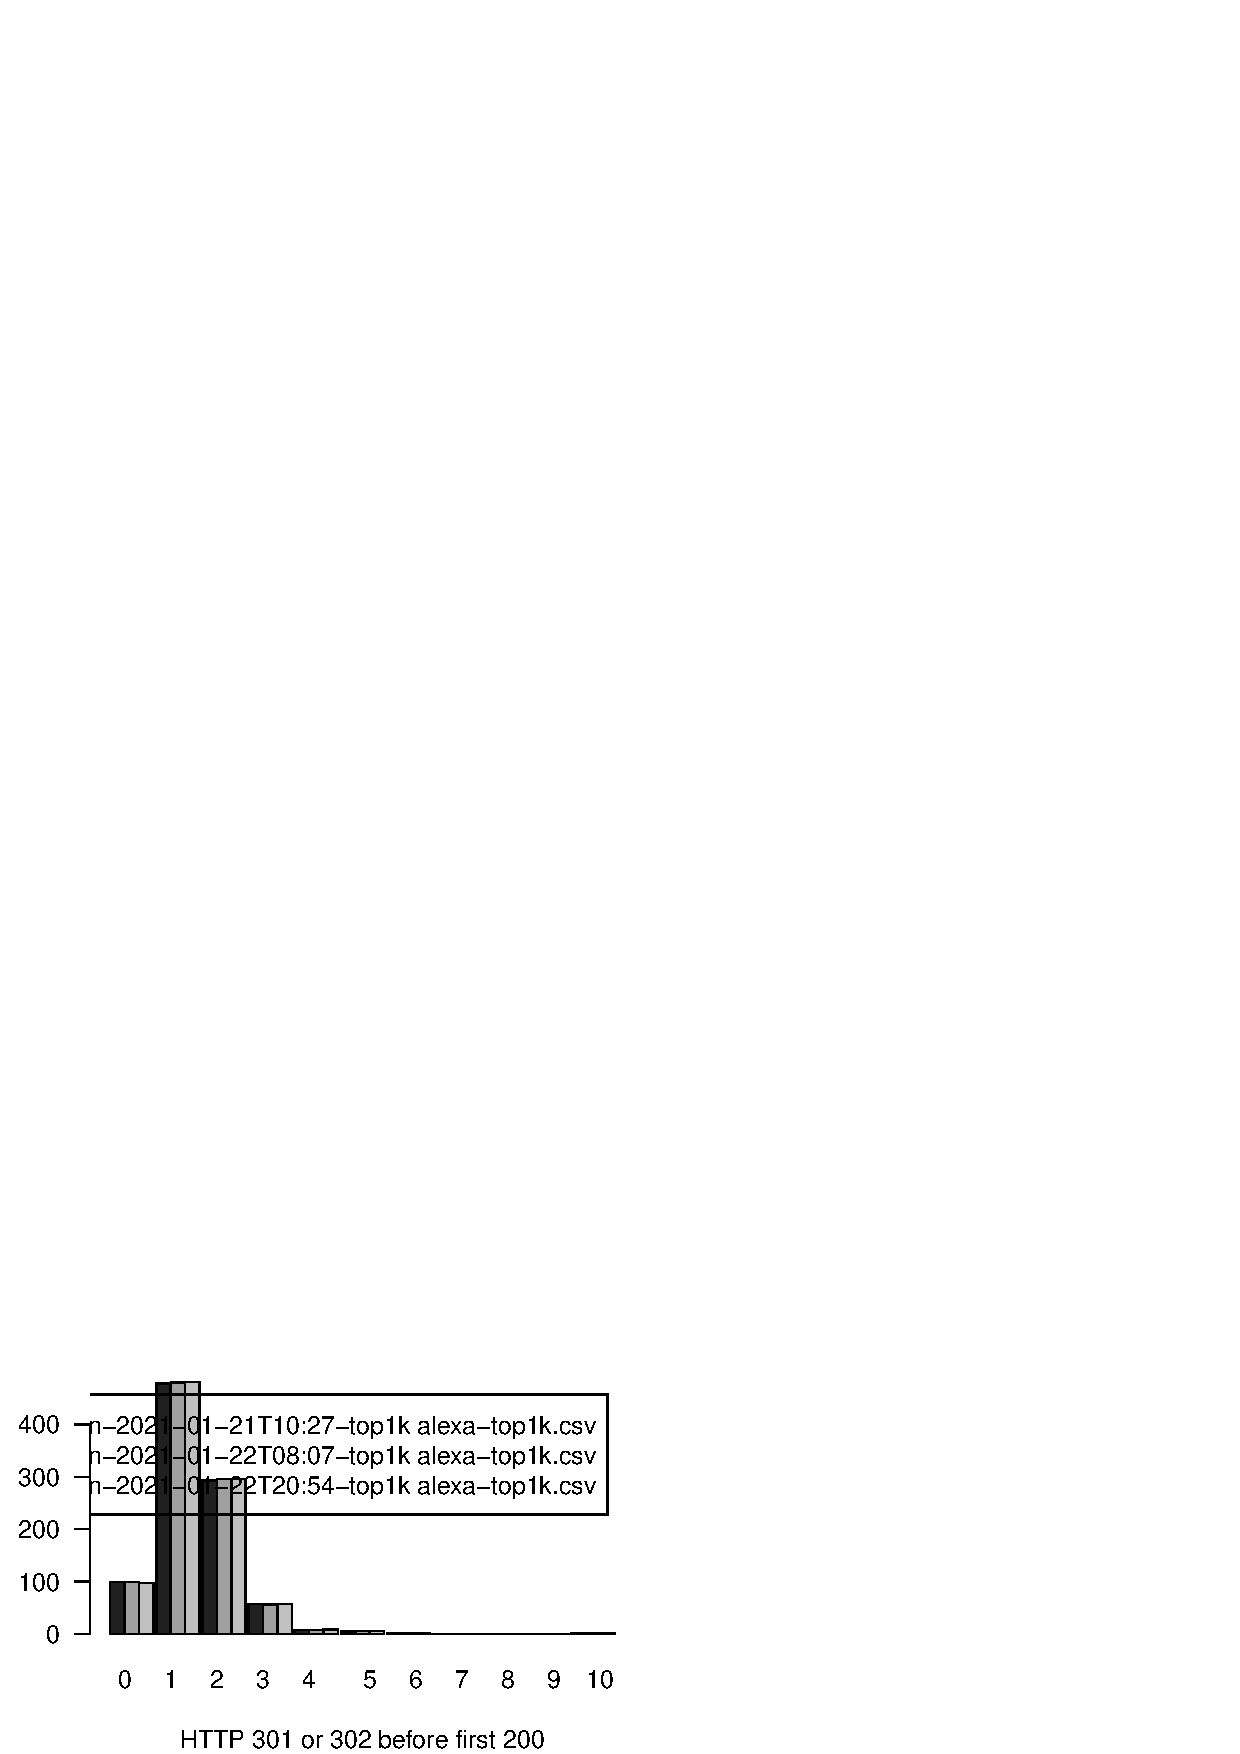
\includegraphics[width=\linewidth]{Original Plots/barplot_redirects.pdf}
	\caption{Original Measurements}
	\label{fig:orig_bar_redirects}
\end{subfigure}
\caption{Number of initial Redirects}
\label{fig:bar_redirects}
\end{figure}

\begin{figure}
 \centering
 \begin{subfigure}{\linewidth}
		\includegraphics[width=\linewidth]{New_Plots/ecdf_loadtimes.pdf}
	\caption{New Measurements}
	\label{fig:new_plot_redirects}
\end{subfigure}\par\medskip
\begin{subfigure}{\linewidth}
		\includegraphics[width=\linewidth]{Original Plots/ecdf_loadtimes.pdf}
	\caption{Original Measurements}
	\label{fig:orig_plot_redirects}
\end{subfigure}
\caption{Page Load Time (PLT) with and without initial redirects}
\label{fig:plot_redirects}
\end{figure}

\subsection{Number and Size of Objects}
In order to estimate the complexity of web pages, metrics such as Object Index, Object Count, and Byte Index are employed. Since web pages are often constantly loading - even after the initial page load - object counts should only count objects loaded by the onLoad event. Calculating a count of the initial objects can be done using objects in the DOM or HTTP request-response pairs. Object size normally reflects the encoded size (i.e. the count of bytes transferred over the network) but can also reflect the decoded (i.e. decompressed) number of bytes. Byte Index refers to the integral of the total sizes of objects loaded over time and is an important metric for the size of Objects \cite{10.1145/2940136.2940138}.

To obtain the number of objects, one can count the number of HTTP request-response pairs in HAR files. The number of objects can also be obtained using the Resource Timings API. Both the Resource Timings API and HAR files supply the encoded and decoded body size. Alternatively, the number of objects can be extracted from packet capture traces if all elements can be decrypted; if this is not the case, object sizes can differ due to TLS padding.
\section{Re-Implementation \& Results}

\begin{frame}
    \frametitle{Re-Implementation Tools}
	\begin{table}
		\centering
		\caption{Comparison Setup \& Tools}
		\label{tab:tools}
		\begin{tabular}{lccccccc}
			\toprule
			& \textbf{Original Paper} & \textbf{Reproduction}\\
			\midrule
			Hardware & Thinkpad L450 & Matebook X Pro (1st Generation)\\
			Operating System & Debian 9 (Stretch) & Ubuntu 20.04\\
			Firefox & 62.0.2 / 61.0.2 & 84.0.2 \\
			Chrome & 69 & 88 \\
			Selenium & 3.14.0 & 3.141.59\\
			Geckodriver & 0.21.0 & 0.29.0\\
			HAR Export Trigger & 0.6.1 & 0.6.1\\
			\bottomrule
		\end{tabular}
	\end{table}
	
Despite trying the versions specified in the original paper as well as the more modern versions, \textbf{it was not possible to consistently extract HAR files using Firefox with Selenium and Chrome with PyDevTools as specified in the original paper}.

$\boldsymbol{\rightarrow}$  This paper focused on reproducing measurements using Firefox with Marionette.
\end{frame}

\begin{frame}
    \frametitle{Results - Redirects}
\begin{figure}
 \centering
 \begin{subfigure}{0.5\textwidth}
 \centering
	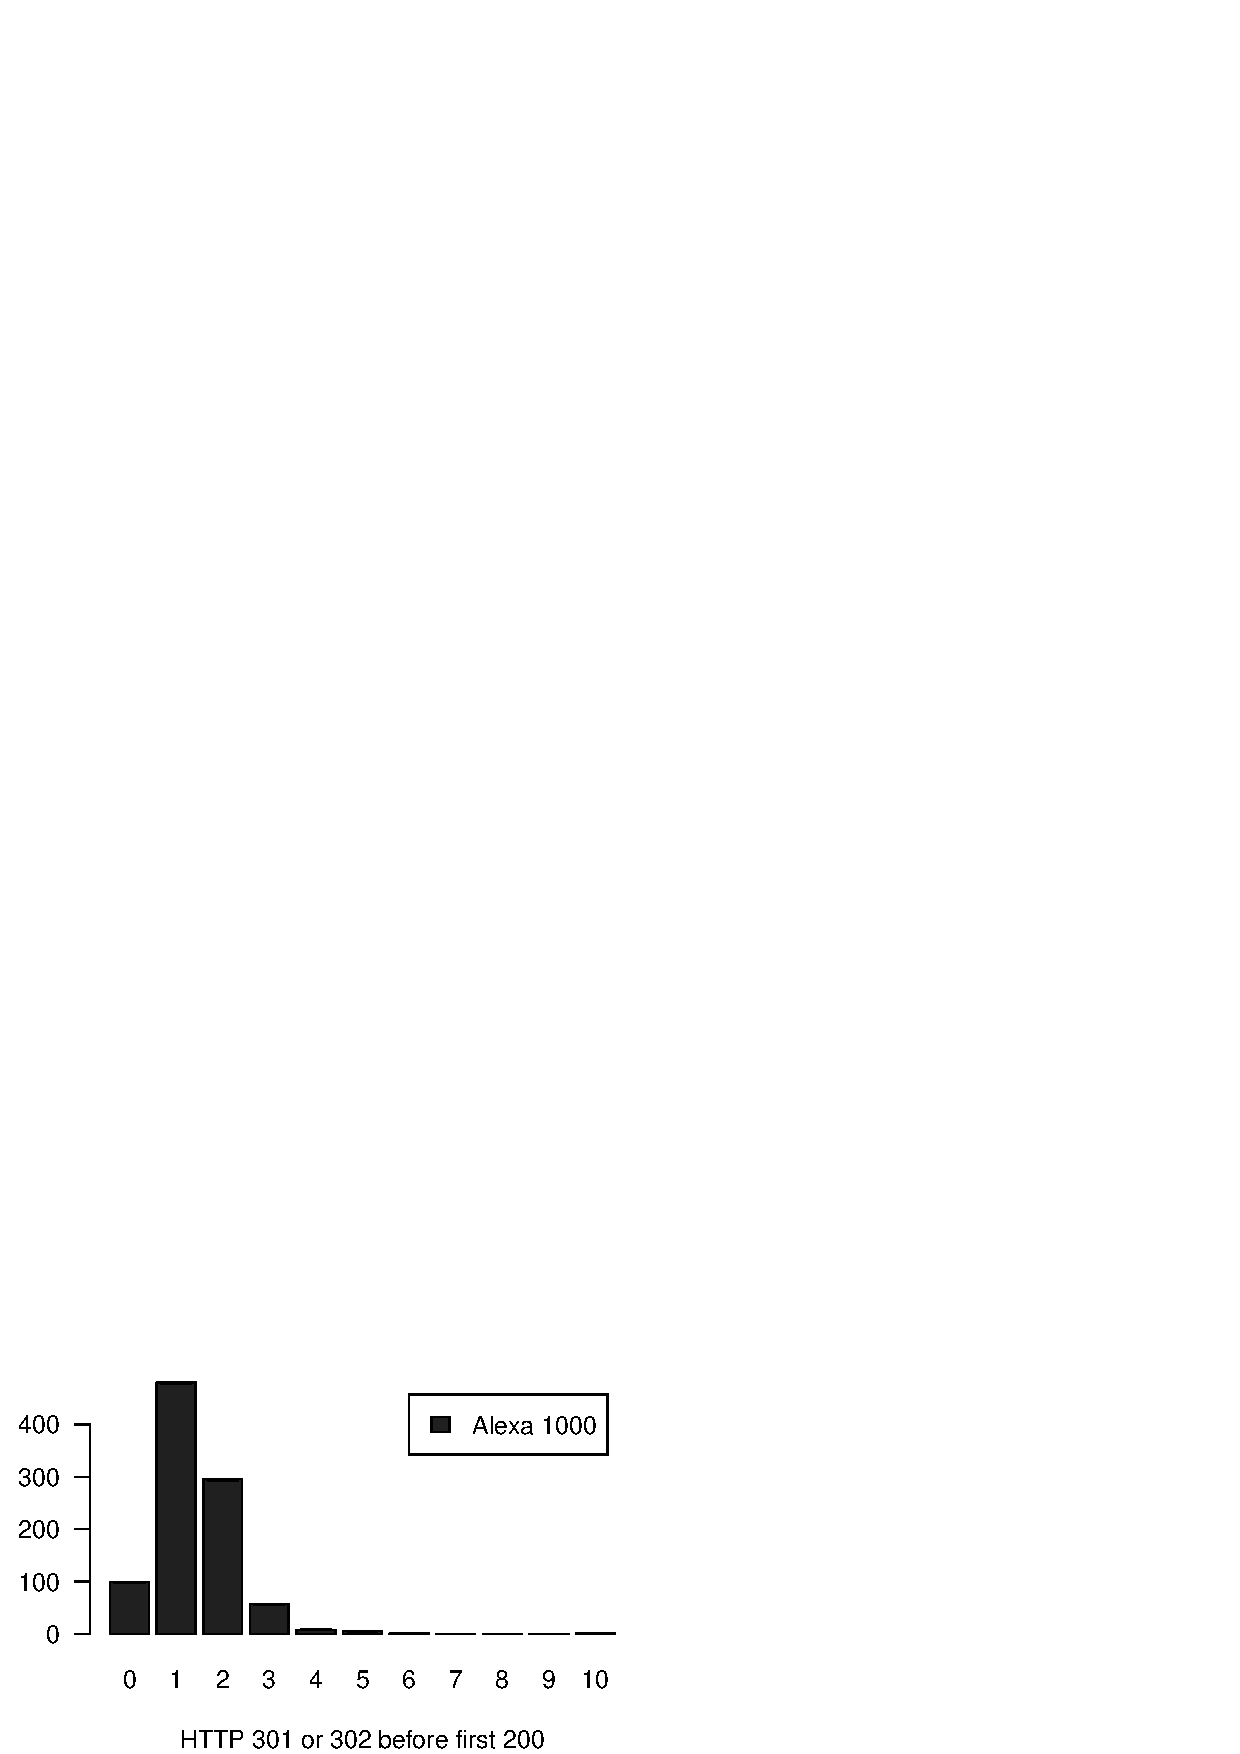
\includegraphics[width=.8\linewidth,keepaspectratio]{New_Plots/barplot_redirects_clean.pdf}
	\caption{New Measurements}
	\label{fig:new_bar_redirects}
	\par\medskip
	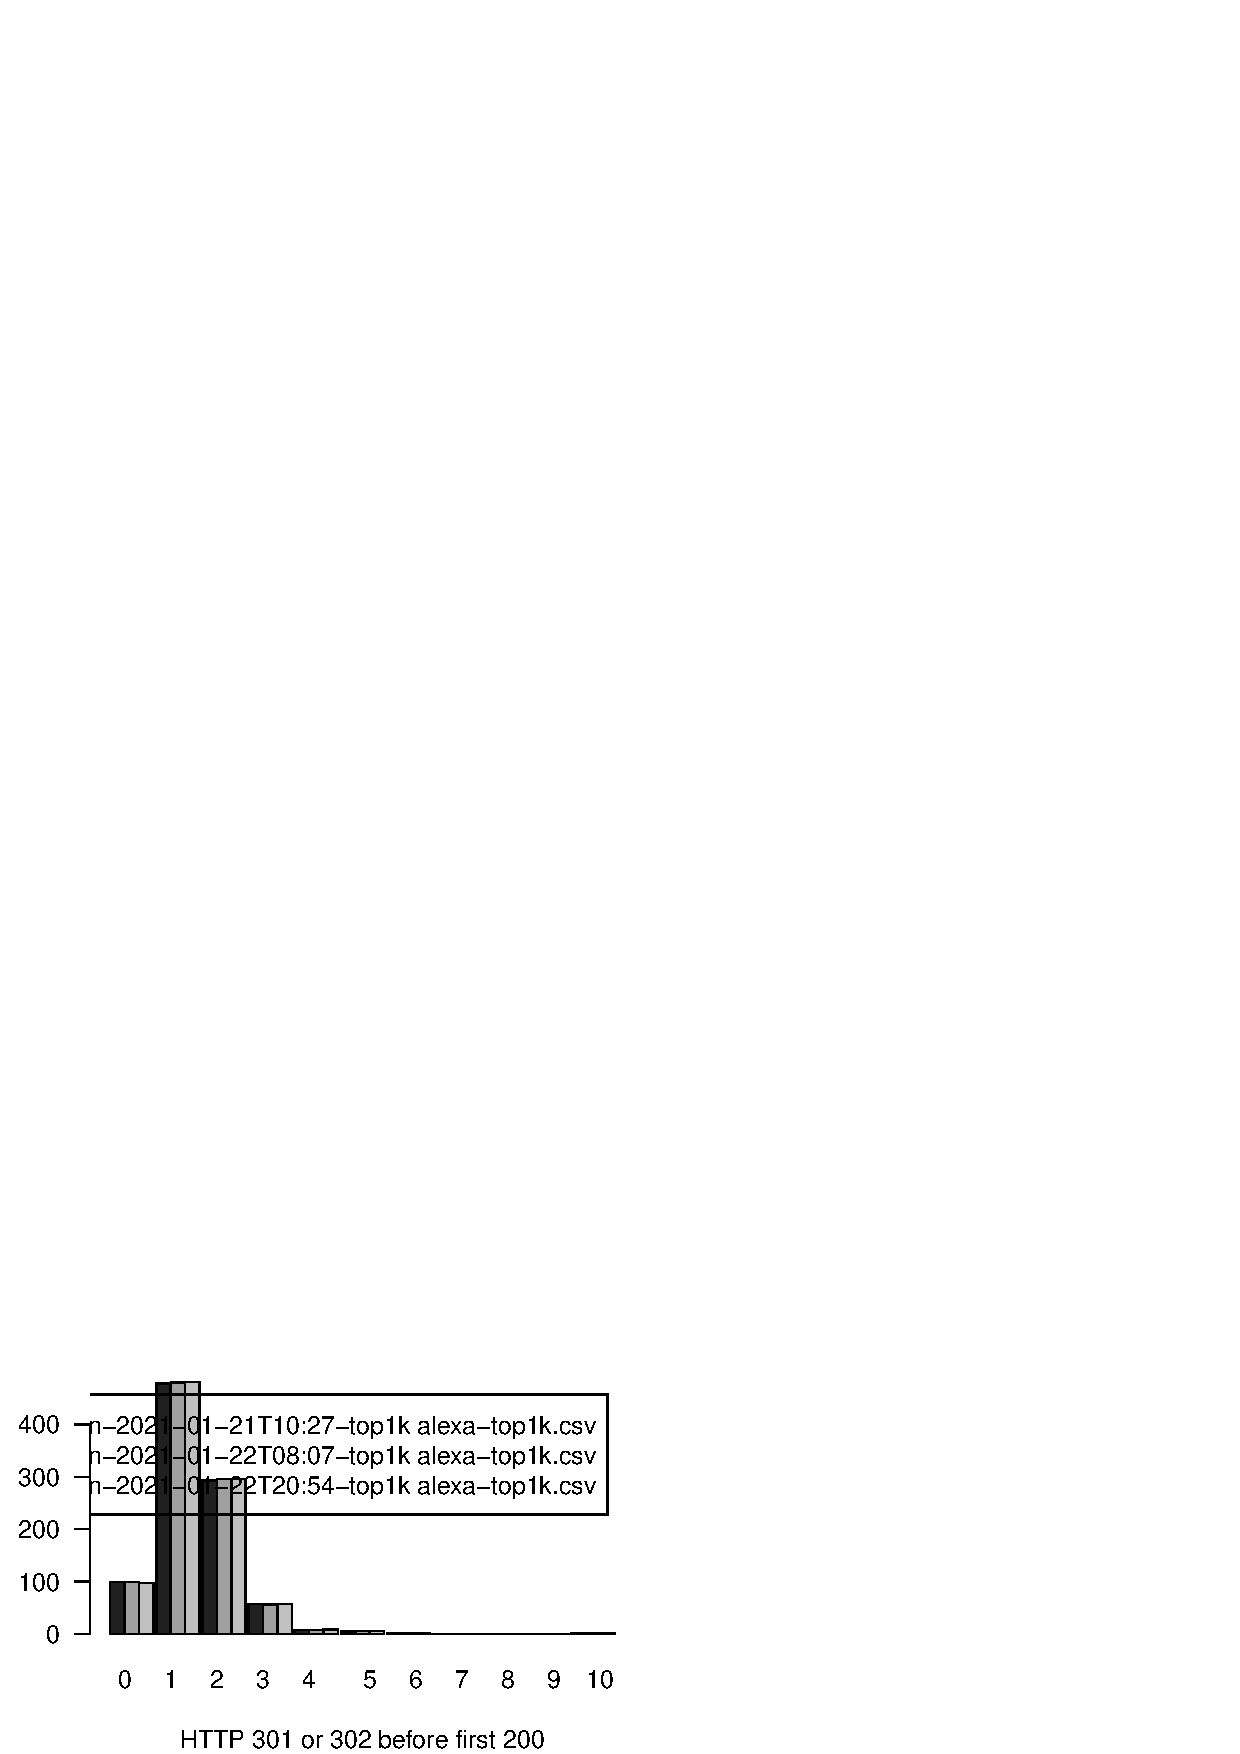
\includegraphics[width=.8\linewidth,keepaspectratio]{Original Plots/barplot_redirects.pdf}
	\caption{Original Measurements}
	\label{fig:orig_bar_redirects}
	\end{subfigure}%
	 \begin{subfigure}{0.5\textwidth}
	 \centering
	\includegraphics[width=.8\linewidth,keepaspectratio]{New_Plots/ecdf_loadtimes.pdf}
	\caption{New Measurements}
	\label{fig:new_plot_redirects}
	\par\medskip
	\includegraphics[width=.8\linewidth,keepaspectratio]{Original Plots/ecdf_loadtimes.pdf}
	\caption{Original Measurements}
	\label{fig:orig_plot_redirects}
	\end{subfigure}
\caption{Number of initial Redirects (Left) \& PLT with and without initial redirects (Right)}
\end{figure}

\end{frame}

\begin{frame}
    \frametitle{Results - Object Sizes}
\begin{figure}
 \centering
 \begin{subfigure}{0.5\textwidth}
 \centering
 	 \includegraphics[width=\linewidth,keepaspectratio]{New_Plots/ecdf_diff_objectsizes.pdf}
	\caption{New Measurements}
	\label{fig:new_absolute_byte_index}
	\end{subfigure}%
	 \begin{subfigure}{0.5\textwidth}
	 \centering
	\includegraphics[width=.8\linewidth,keepaspectratio]{Firefox Plots/ecdf_diff_objectsizes.pdf}
	\caption{Original Measurements (Firefox Only)}
	\label{fig:orig_absolute_byte_index}
	\par\medskip
	\includegraphics[width=.8\linewidth,keepaspectratio]{Chrome_Plots/ecdf_diff_objectsizes.pdf}
	\caption{Original Measurements (Chrome Only)}
	\label{fig:orig_chrome_absolute_byte_index}
	\end{subfigure}
\caption{Object sizes: differences due to metric for all objects}
\end{figure}

\end{frame}


\begin{frame}
    \frametitle{Results - Object Counts / Byte Index}
\begin{figure}
 \centering
 \begin{subfigure}{0.5\textwidth}
 \centering
 	 \includegraphics[width=\linewidth,keepaspectratio]{New_Plots/ecdf_rel_object_byte_index.pdf}
	\caption{New Measurements}
	\label{fig:new_relative_byte_index}

	\end{subfigure}%
	 \begin{subfigure}{0.5\textwidth}
	 \centering
	\includegraphics[width=.8\linewidth,keepaspectratio]{Firefox Plots/ecdf_rel_object_byte_index.pdf}
	\caption{Original Measurements (Firefox Only)}
	\label{fig:orig_firefox_relative_byte_index}
		\par\medskip
		\includegraphics[width=.8\linewidth,keepaspectratio]{Chrome_Plots/ecdf_rel_object_byte_index.pdf}
	\caption{Original Measurements (Chrome Only)}
	\label{fig:orig_chrome_relative_byte_index}
	\end{subfigure}
\caption{Byte index: difference due to data source}
\end{figure}

\end{frame}

\section{Conclusion}

\begin{frame}
    \frametitle{Analysis}
	This reproducibility report shows the following: 
	\begin{itemize}
        \item The new dataset contradicts the conclusion in the original paper that the Content-Length in HAR files is the most reliable data source for object sizes but does confirm the large inconsistencies in object size between data sources.
        \item The other examined conclusions regarding redirects and object count / byte index were confirmed by the new dataset.
        \item The data in both papers underlines the importance of improving the documentation of studies of web performance as well as choosing performance metrics carefully and deliberately. 
   	 \end{itemize}
\end{frame}

\begin{frame}
    \frametitle{Questions?}
      \centering \Large
  	\emph{Thank you for your attention!}
  	
  	Please feel free to ask questions now or contact me after the talk:
    
    \textbf{Curt Polack}
    
    \textbf{curt.polack@tum.de}
    
    
\end{frame}


% Include markdown source from ./pandoc
%\input{pandoc/example}

% Comment out if you do not want a bibliography
\section{Bibliography}
\begin{frame}[allowframebreaks]
    \bibliographystyle{abbrv}
    \setbeamertemplate{bibliography item}[text]
    \footnotesize
    \bibliography{lit}
\end{frame}

\end{document}

